% Template LaTeX para Informes de Proyectos de Grado de Computación
% InCo, Facultad de Ingeniería, Universidad de la República
% 06/2023


\documentclass{prgrado}
\usepackage[colorinlistoftodos]{todonotes}
\usepackage{siunitx}
\usepackage{booktabs} 
\usepackage{glossaries}
\usepackage[utf8]{inputenc}
\makeglossaries

% título del proyecto (debe escribirse en minúscula, con excepción de la
% letra inicial de la primera palabra y nombres propios)
\title{Módulo de inteligencia artificial generativa basado en OpenFing}                   

% autores
\author{Diego Amorena, Guido Dinello}  

% fecha de la defensa
\date{\today}                                 

\supervisor{Luis Chiruzzo}              
\cosupervisor{Libertad Tansinni}

% licencia creative commons del documento
% opciones: by, by-sa, by-nd, by-nc, by-nc-sa y by-nc-nd
% opción por defecto: by-nc-nd versión 4.0
\cclicense{by}{4.0}

%%%%%%%%%%%%%%%%%%%%%%%%%%%%%%%%%%%%%%%%%%%%%%%%%%%%%%%%%%%%%%%%%%%%%%%%%%%%%%%%%%%%%%%%%%%%%%%%


%links con colores 
\hypersetup{
  colorlinks   = true,
  urlcolor     = blue,
  linkcolor    = blue,
  citecolor    = red
}
%%%%%%%%%%%%%%%%%%%%%%%%%%%%%%%%%%%%%%%%%%%%%%%%%%%%%%%%%%%%%%%%%%%%%%%%%%%%%%%%%%%%%%%%%%%%%%%%
% TODO: Pasar esto a un archivo aparte asi no jode.
\newglossaryentry{prompt}
{
    name=consigna (prompt),
    description={Instrucción o texto de entrada en lenguaje natural que se proporciona a un modelo de lenguaje para orientar su respuesta. Es el mecanismo fundamental de interacción con los modelos de lenguaje de gran escala}
}

\newglossaryentry{chunk}
{
    name=fragmento (chunk),
    description={Segmento de texto de longitud controlada en el que se divide un documento extenso. Esta técnica permite procesar información dentro de los límites de memoria de los modelos de lenguaje}
}

\newglossaryentry{embedding}
{
    name=representación vectorial (embedding),
    description={Codificación de texto en un vector numérico de alta dimensionalidad que captura relaciones semánticas. Permite realizar búsquedas por similitud de conceptos en lugar de coincidencias exactas de palabras}
}

\newglossaryentry{token}
{
    name=unidad léxica (token),
    description={Unidad mínima de procesamiento en un modelo de lenguaje. Puede representar palabras, subpalabras o caracteres, dependiendo del algoritmo de tokenización}
}

\newglossaryentry{contexto}
{
    name=ventana de contexto,
    description={Límite máximo de información (medido en unidades léxicas) que el modelo puede procesar de forma simultánea en una sola interacción}
}

\newglossaryentry{Inferencia}
{
    name=inferencia,
    description={Fase en la que un modelo ya entrenado genera predicciones o respuestas ante nuevos datos de entrada}
}

\newglossaryentry{Fine-Tuning}
{
    name=ajuste fino (fine-tuning),
    description={Proceso de especialización de un modelo preentrenado mediante un entrenamiento adicional con un conjunto de datos específico para una tarea o dominio particular}
}

\newglossaryentry{alucinación}
{
    name=alucinación,
    description={Error semántico donde el modelo genera información que es gramaticalmente correcta pero factual o lógicamente falsa}
}

\newglossaryentry{Temperatura}
{
    name=temperatura,
    description={Parámetro de configuración que regula el grado de aleatoriedad en la generación de texto. Valores bajos favorecen la precisión y valores altos la creatividad}
}

\newglossaryentry{API}
{
    name=interfaz de programación (API),
    description={Siglas de \textit{Application Programming Interface}. Conjunto de protocolos que permite la comunicación y el intercambio de datos entre diferentes componentes de software}
}

\newglossaryentry{Vectordb}
{
    name=base de datos vectorial,
    description={Sistema de almacenamiento especializado para gestionar vectores de alta dimensionalidad (\textit{embeddings}), permitiendo búsquedas de similitud semántica a gran escala}
}

\newglossaryentry{Transcripción}
{
    name=transcripción (ASR),
    description={Proceso de conversión de señal de audio a texto escrito mediante reconocimiento automático de voz (\textit{Automatic Speech Recognition})}
}

\newglossaryentry{Accuracy}
{
    name=exactitud (accuracy),
    description={Métrica que cuantifica la proporción de aciertos totales realizados por el modelo sobre el conjunto de pruebas}
}

\newglossaryentry{frontend}
{
    name=interfaz de usuario (front-end),
    description={Capa de presentación de la aplicación con la que el usuario interactúa. Incluye el diseño visual y la lógica de cliente}
}

\newglossaryentry{backend}
{
    name=lógica de servidor (back-end),
    description={Capa de acceso a datos y procesamiento lógico que se ejecuta en el servidor y da soporte a la interfaz de usuario}
}

% Conceptos que mantienen su nombre propio comercial
\newglossaryentry{react}
{
    name=React,
    description={Biblioteca de JavaScript para la construcción de interfaces de usuario basadas en componentes}
}

\newglossaryentry{nodejs}
{
    name=Node.js,
    description={Entorno de ejecución de JavaScript en el servidor basado en el motor V8}
}

\newglossaryentry{OpenFing}
{
    name=OpenFing,
    description={Plataforma educativa de la Facultad de Ingeniería (UdelaR) que brinda acceso abierto a grabaciones de cursos de grado}
}

%%%%%%%%%%%%%%%%%%%%%%%%%%%%%%%%%%%%%%%%%%%%%%%%%%%%%%%%%%%%%%%%%%%%%%%%%%%%%%%%%%%%%%%%%%%%%%%%
% Acrónimos (Siglas en inglés con expansión en español)
%%%%%%%%%%%%%%%%%%%%%%%%%%%%%%%%%%%%%%%%%%%%%%%%%%%%%%%%%%%%%%%%%%%%%%%%%%%%%%%%%%%%%%%%%%%%%%%%

\newacronym{llm}{LLM}{Modelo de Lenguaje de Gran Escala (\textit{Large Language Model})}
\newacronym{rag}{RAG}{Generación Aumentada por Recuperación (\textit{Retrieval-Augmented Generation})}
\newacronym{nlp}{PLN}{Procesamiento de Lenguaje Natural (conocido como \textit{NLP})}
\newacronym{asr}{ASR}{Reconocimiento Automático de Voz (\textit{Automatic Speech Recognition})}
\newacronym{ia}{IA}{Inteligencia Artificial}
\newacronym{json}{JSON}{\textit{JavaScript Object Notation}}
\newacronym{http}{HTTP}{\textit{Hypertext Transfer Protocol}}
\newacronym{url}{URL}{\textit{Uniform Resource Locator}}
\newacronym{csv}{CSV}{\textit{Comma-Separated Values}}
\newacronym{ui}{IU}{Interfaz de Usuario (\textit{User Interface})}
\newacronym{ux}{EX}{Experiencia de Usuario (\textit{User Experience})}
% carátula

\begin{document}

\maketitle


\frontmatter % numeración en romanos, capitulos sin numerar

\todo[color=yellow, inline, list]{
Cambios Realizados desde la versión anterior:

    Se movio el Resumen a antes que lo agradecimientos. 
    
    Se refencia a la herramienta como el Asistente. 

    
    Dentro de: 
        Resumen, ligeros detalles modificados.
        Introducción: sin cambios.

        
    Marco Teórico: 
Se añadió una intro al capitulo. 
Se añadio referencias de Jurasky en Inteligencia artificial y Redes Neuronales


              
        Correciones realizadas en sección inteligencia artificial generativa.
        
    
}

\chapter*{Resumen}
\label{chapter:0-Resumen}

La inteligencia artificial generativa ha transformado diversos ámbitos y áreas. Un campo particularmente impactado es la educación superior. En búsqueda de un aprendizaje más eficiente y accesible, los estudiantes recurren y consultan cada vez más a grandes modelos de lenguaje (LLMs) y otras herramientas de inteligencia artificial generativa para complementar sus estudios y resolver dudas académicas. Sin embargo, los modelos comerciales funcionan como cajas negras y su uso conlleva ciertos riesgos, por lo que surge la necesidad de proveer a los estudiantes de la FING una solución personalizada que mitigue esos riesgos.

En este documento se presenta el diseño, la implementación y la evaluación de un asistente de inteligencia artificial generativa orientado a estudiantes de la Facultad de Ingeniería (FING) de la Universidad de la República (UdelaR). El asistente implementado de inteligencia artificial generativa se basa en la arquitectura de Generación Aumentada por Recuperación (RAG) y se utilizan como corpus de conocimiento los videos a las clases publicadas en OpenFing. Para ello, se desarrolló un pipeline automatizado con el objetivo de transcribir mediante herramientas de reconocimiento automático de voz (ASR) el contenido de estas clases. 

A su vez, se presenta la arquitectura final del sistema junto con las alternativas consideradas y los motivos por los que se dejaron de lado. También se expone la experimentación asociada a cada etapa del diseño del asistente. 


\hfill \break
\keywords{RAG, LLM, OpenFing, ASR, Educación}

%%%%%%%%%%%%%%%%%%%%%%%%%%%%%%%%%%%%%%%%%%%%%%%%%%%%%%%%%%%%%%%%%%%%%%%%%%%%%%%%%%%%%%%%%%%%%%%%




\chapter*{Agradecimientos}

Agradecer, siempre es bueno agradecer%.Agradecemos a nuestro supervisor Luis Chiruzzo por su guía y apoyo constante a lo largo de este proyecto. También extendemos nuestro agradecimiento a Libertad Tansinni, nuestra cosupervisora, por sus valiosas aportaciones y orientación.
\printglossaries

\mainmatter

\chapter{Introducción}
\label{chapter:1-Introducción} 

%\textit{Aquí se motiva el trabajo, se plantea y define el problema, se deja claro cuales son los objetivos (general del proyecto, si correspondiese o si está inmerso en un proyecto de mayor alcance, y los específicos), se plantean los resultados esperados, se establecen resumidamente las conclusiones y se describe la organización general del documento.
% Este y los siguientes capítulos pueden incluir referencias, algunos ejemplos de referencias pueden ser \cite{CitekeyArticle}, \cite{CitekeyBook}, \cite{CitekeyInproceedings}, \cite{CitekeyManual} y \cite{CitekeyMisc}. Se sugiere citar usando el formato APA.}
%En la introducción se deberá:
%Explayar el resumen previo. 
%Explicar en detalle algunas de las %posibles falencias que se basan en %utilizar modelos que no fueron entrenados %con contenido educativo o que no fueron %entrenados con contenido local/regional.
%Ej.:
%nombres, enfoques o convenciones distintos %que nosotros (UdelaR o Uruguay) podamos %usar en comparación con un ámbito %internacional.
%Un caso de valor puede ser que el Método %Simplex (Introducción a la Investigación %Operativa) se dé de manera distinta.
%
Se deberá detallar el scope del proyecto, el alcance que nos propusimos.
Se deberá detallar cada uno de los parámetros de entrada y de los parámetros que se investigaron y evaluaron para llegar a un mejor resultado.
Se deberá detallar en base a qué evaluamos un modelo / un resultado como mejor o peor que otro.

--Lo Siguiente ya estaba escrito--

El acceso a información confiable y relevante es un desafío constante para los estudiantes universitarios. Aunque las grabaciones de clase pueden ser una herramienta útil, presentan varias limitaciones: su consumo es lento, pueden contener problemas de audio que dificultan la comprensión, y en muchos casos, solo una fracción del contenido resulta realmente valiosa. Además, la información presentada en clase puede quedar desactualizada con el tiempo, lo que genera confusión y dificulta el aprendizaje efectivo.

Este trabajo de tesis se centra en el desarrollo de un producto basado en el fine-tuning de un modelo de lenguaje (LLM) con contenido educativo específico de una facultad, utilizando como fuente principal las grabaciones de las clases. El objetivo es ofrecer a los estudiantes una herramienta en formato de pregunta-respuesta que les permita acceder rápidamente a información precisa y relevante, directamente basada en sus propias clases.

La implementación de esta solución no solo agiliza el proceso de aprendizaje, sino que también proporciona un medio más eficiente para digerir la información. Los estudiantes podrán realizar consultas en tiempo real sobre el contenido de sus cursos, sin necesidad de revisar extensos videos o depender de fuentes externas cuya fiabilidad puede ser incierta. De esta manera, se garantiza que el conocimiento adquirido provenga de una fuente validada y alineada con el plan de estudios de la facultad.

Este enfoque representa un avance significativo en la optimización del aprendizaje, brindando a los estudiantes una alternativa moderna y efectiva para complementar su formación académica.

\section{Objetivos del Proyecto}
\label{section:1-Objetivos del Proyecto}


\section{Resultados Obtenidos}
\label{section:1-Resultados Obtenidos}


\section{Organización del Documento}
\label{section:1-Organización del Documento}

El proximo documento se estructura de la siguiente manera:

\autoref{chapter:2-Marco Teórico} 
En este capítulo se presenta una revisión del estado del arte, los conceptos teóricos relevantes que sustentan el desarrollo del proyecto y una descripción para familiarizar al lector con OpenFing.

\autoref{chapter:3-Requisitos del Sistema} 
En este capítulo se formalizan los requisitos funcionales y no funcionales del sistema propuesto. 

\autoref{chapter:4-Arquitura y Diseño} 
En este capítulo se expone la arquitectura general del sistema y el diseño detallado de sus componentes. Se presentan diagramas de arquitectura y flujos de datos.

\autoref{chapter:5-Implementación} 
En este capítulo se describe las  implementación del sistema, las tecnologías utilizadas y sus expectativas.

\autoref{chapter:6-Experimentación} 
En este capítulo se presentan los experimentos realizados para evaluar el desempeño del sistema. Se describen los conjuntos de datos utilizados, las métricas de evaluación, y los resultados obtenidos. 

\autoref{chapter:7-Trabajo a futuro} 
En este capítulo se exploran las posibles direcciones futuras mejoras del sistema. 

\autoref{chapter:8-Conclusiones} 
En este capítulo se resumen los principales hallazgos del proyecto y se reflexiona sobre el cumplimiento de los objetivos planteados. 
\chapter{Marco Teórico}
\label{chapter:2-Marco Teórico} 
\todo[inline,color=cyan]{TODO: verificar y Cambiar todas las fuentes a Articulos cientificos}

En el marco teórico se amplía el contexto actual mencionado previamente, se explican algunos de los conceptos relevantes y necesarios para un apropiado entendimiento del proyecto y también se evalúan algunos proyectos similares al mismo en los que el grupo tomó inspiración en ciertas cuestiones. 

\section[OpenFING]{OpenFing}
\label{section:2-OpenFING}
Como se explicó anteriormente, el proyecto de grado se depende activamente de \Gls{OpenFing} cómo base de conocimiento. En está sección se explicá el origen y el rol actualmente en la facultad.
\Gls{OpenFing} es una plataforma de videos educativos de la Facultad de Ingeniería de la Universidad de la República (UdelaR). La plataforma permite que profesores suban clases, para facilitar el seguimiento de los cursos de la FING. Provee la difusión y el acceso de las clases de la institución más allá de la presencialidad.

En 2012 se creó como una herramienta de estudio complementaria para repasar contenidos desarrollados en clases presenciales. Hoy en día, cuenta con más de 5000 horas de video, más de 3000 clases subidas. Además, casi todos los cursos se apoyan en mayor o menor medida en \Gls{OpenFing}, consolidándola como un pilar del aprendizaje digital dentro de la institución. Para la realización de este proyecto se transcribieron todas las clases incluidas en esta plataforma.

Actualmente la plataforma no solo se utiliza para repasar las clases presenciales como antes. En ocasiones los cursos sustituyen completamente el dictado de clases presenciales por las clases ya previamente subidas en \Gls{OpenFing}. Por ejemplo el curso de Programación 2 únicamente dicta clases practicas presenciales y no dicta clase teoricas. De está manera, OpenFING toma un rol importante en descentralización del acceso a la educación superior. Los estudiantes que residen en el interior del país pueden seguir las clases, mantenerse actualizados y sentirse parte activa de la comunidad universitaria, sin que la distancia con Montevideo sea una barrera. Así, \Gls{OpenFing} no solo facilita el aprendizaje, sino que también contribuye a la inclusión y a la democratización del conocimiento, extendiendo el alcance de la Facultad de Ingeniería más allá de sus fronteras físicas.

El grupo aspira a que el proyecto de grado actual pueda aportar de manera similar a lo que \Gls{OpenFing} aportó a la facultad, e impactó las carreras universitarias de muchos estudiantes. 

\cite{OpenFing}
\todo[inline]{Todo: arreglar problema con las referencias, este problema aparece en todas las referencias}

\section{Conceptos Generales}
\label{section:2-Conceptos Generales}
En está sección se encuentra las explicaciones de los conceptos vitales para el entendimiento del proyecto. 





\subsection{Inteligencia artificial}
\label{subsection:2-Inteligencia artificial}


La inteligencia artificial (IA) es un campo de la informática orientado a la creación de sistemas capaces de realizar tareas que habitualmente requieren inteligencia humana. Según \cite{RussellNorvig2020}, se encuentran dos ejes dentro de las definiciones tradicionales de la disciplina: uno plantea la distinción el pensamiento interno y el comportamiento externo, y otro que diferencia entre el cómo actúan y se desempeñan los humanos y la racionalidad.

En los últimos años se ha popularizado una rama especifica de la IA, que es la Inteligencia artificial generativa. Es la idea de utilizar IA para producir texto, imágenes, código, videos, etc.
Anteriormente, el procesamiento de lenguaje natural se realizaba mayormente con el enfoqué del entendimiento texto, esto cambia con la popularización de los LLMs.

\cite{InteligenciaArificialGenerativa}

\todo[inline]{ TODO: Seccion de NLP}

\subsection{Red Neuronal}
\label{subsection:2-Red Neuronal}

Una red neuronal es una estructura algorítmica inspirada en el funcionamiento del cerebro humano, compuesta por nodos (neuronas artificiales) interconectados en capas. Estas redes \"aprenden\" patrones complejos a través del ajuste iterativo de pesos matemáticos durante el entrenamiento. Cuando una red neuronal tiene múltiples capas ocultas, se denomina red neuronal profunda (deep neural network), y es la base de técnicas como el deep learning, que permite el procesamiento de datos a gran escala, como en los LLM.

\todo[inline]{Jurasky explica que es red neuronal, goodwill explica qué es deeplearning.}

\cite{Jurafsky2023} 

\cite{Goodfellow-et-al-2016}


\subsection{Tokenización}
\label{subsection:2-Tokenización}
La tokenizacion es el proceso de dividir texto en unidades de secciones más pequeñas. Cada una de estas secciones las llamamos tokens. Un \gls{token} puede ser una palabra, varias palabras juntas, una única silaba de una palabra o incluso una única letra de una palabra. Esto varía dependiendo de la estrategia de tokenización. Con motivo de simplificación se explicarán futuros conceptos utilizando token como equivalente a una única la palabra dentro de un texto.

\cite{Jurafsky2023}

\subsection{Modelo de lenguaje y LLMS}
\label{subsection:2-Modelo de lenguaje y LLMS}

Un modelo de lenguaje es un sistema de inteligencia artificial entrenado para predecir la siguiente palabra (o \gls{token}) a partir de una secuencia de entrada. Esta tarea de predicción de la 
siguiente palabra constituye fundamentalmente el entrenamiento de los modelos de lenguaje de última generación. Diseñados para comprender y generar texto de manera coherente. Estos modelos se entrenan utilizando grandes volúmenes de datos textuales, con el objetivo de identificar patrones y relaciones entre palabras y frases. Así, al recibir una secuencia de palabras —por ejemplo, un \gls{prompt} de un usuario (explicado en la sección \autoref{subsection:2-prompt})— el modelo es capaz de producir una continuación coherente y contextualizada. De este modo, resulta posible realizar tareas como responder preguntas o mantener conversaciones de manera natural.

\cite{Modelos_De_Lenguage}

Los grandes modelos de lenguaje (LLMs, por sus siglas en inglés) se distinguen de los modelos anteriores principalmente por su mayor complejidad y capacidad de procesamiento. Estos sistemas son entrenados con volúmenes masivos de datos textuales. Esto permite captar patrones lingüísticos más amplios y profundos. Gracias a ello, son capaces de comprender mejor el lenguaje natural y generar texto coherente, incluso en contextos genéricos o no especializados.
Además, los LLMs presentan arquitecturas significativamente más sofisticadas, compuestas por millones —e incluso miles de millones— de parámetros. Esta escala les otorga una notable capacidad para modelar relaciones semánticas complejas y adaptarse a una amplia variedad de tareas de procesamiento del lenguaje natural, superando ampliamente las limitaciones de los modelos más pequeños o específicos.

\cite{SpeechandLanguageProcessing}
\cite{Diferencia_LLMS_y_Modelos_De_Lenguaje}

\subsection{Segmentos}
\label{subsection:2-Segmentos}

Los textos utilizados por los LLMs pueden ser de cualquier largo, pero
textos largos no son convenientes debido a que son más complejos de procesar que textos más cortos. Por eso los textos con los que los LLMs se entrenan se dividen en secciones más pequeñas, favoreciendo un procesamiento de texto más efectivo sin que se pierdan detalles importantes de la información provista.

\cite{chunks} 


El cómo generar estas secciones individuales se determina a partir de la estrategia de \textit{chunking} (fragmentación, en español) utilizada, y a cada sección individual se le denomina como \textit{\gls{chunk}}.

\subsubsection{Segmentos Semánticos}
\label{subaubsection:2-Semantic Chunks}
\label{subsection:2-Semantic Chunks}
\todo[inline,color=cyan]{alargar}


Hay diferentes tipos de estrategias de chunking.
La estrategia utilizada en este proyecto se la llama Chunking semántico. Dicha estrategia busca segmentar el contenido en función del tema o idea principal abordada en cada porción de texto. Se intenta  preservar coherencia semántica en cada uno de los chunks y evitar la división de oraciones o ideas relacionadas en chunks distintos. \cite{Jurafsky2023}

\subsection[Prompt]{\Gls{prompt}}
\label{subsection:2-prompt}

En el \gls{contexto} de LLMs, se conoce como \textit{\gls{prompt}} a la instrucción o pregunta del usuario al modelo. La estructura específica de un \gls{prompt} afecta significativamente la respuesta del modelo.

Los prompts que obtienen mejores resultados son aquellos apropiadamente estructurados. Según \cite{Prompts_y_estrategia_de_prompts}, los mejores prompts incluyen la petición requerida, instrucciones o el paso a paso para realizar dicha petición, el \gls{contexto} en que se precisa, el rol que el modelo cumple dentro del \gls{contexto} o algún ejemplo de la petición realizada. 

Los siguientes son ejemplos sacados del mismo articulo.


\begin{figure}[htbp]
    \centering
    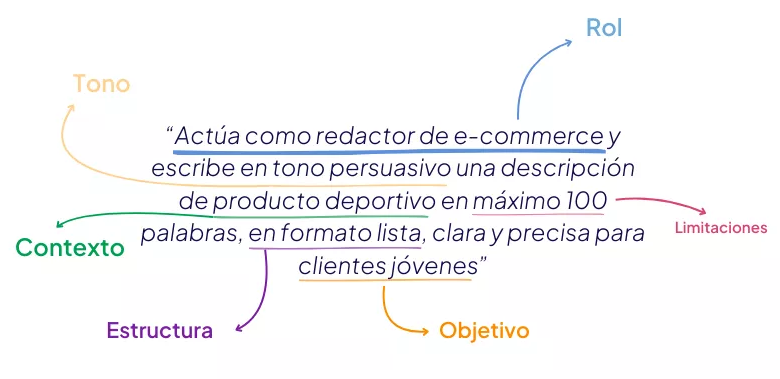
\includegraphics[width=0.8\linewidth]{Nuestro/Imagenes/Figuras_De_Articulos/que_es_un_prompt_infografia.png}
    
    \caption{Ejemplo de \gls{prompt}}
    \label{fig:2-2-5-que_es_un_prompt_infografia}
\end{figure}

“Actúa como un especialista en redes sociales. Diseña un calendario de 5 publicaciones para Instagram sobre [INSERTAR PRODUCTO], indicando tipo de post, copy y objetivo de cada publicación.”


La técnica de proveer ejemplos dentro del \gls{prompt} se conoce como \textit{Few-Shot Prompting}. En contraparte, la técnica \textit{Zero-Shot Prompting} consiste en no proveer ningún ejemplo dentro de la instrucción. En particular, la \textit{One-Shot Prompting} permite al modelo generalizar a partir de un único ejemplo. La siguiente es una explicación de la técnica de  \cite{One_Shot_Prompting}.

"Esta estrategia es útil cuando no es posible disponer de grandes volúmenes de datos de entrenamiento. Los modelos de lenguaje, como GPT-4 o Granite, generalicen eficazmente a partir de un único ejemplo, logrando resultados coherentes con un esfuerzo mínimo en la preparación de datos. Además, facilita el diseño rápido de tareas nuevas y mejora la adaptación del modelo a contextos específicos sin necesidad de reentrenamiento."


Estas técnicas se utilizan en el proyecto. 


\subsection[Embedding]{\Gls{embedding}}
\label{subsection:2-embedding}

\cite{Jurafsky2023}
\subsection{Alucinaciones en Modelos de Lenguaje}
\label{subsection:2-Alucinaciones en Modelos de Lenguaje}

Las alucinaciones en modelos de lenguaje grandes (LLMs) representan un desafío crítico en aplicaciones que requieren precisión factual. Una alucinación es cuando un modelo de lenguange produce contenido plausible pero incorrecto, inconsistente o enteramente fabricado. Los modelos de lenguaje presentan dicho contendo con confianza, lo que induce a los usuarios a creer en la veracidad de la información. 

Las alucinaciones ocurren principalmente por tres factores: primero, los LLMs son modelos probabilísticos entrenados para predecir secuencias de tokens verosímiles, no necesariamente verídicas; segundo, la información en sus parámetros puede estar desactualizada o ser incompleta; tercero, durante situaciones de incertidumbre, el modelo tiende a completar patrones lingüísticos coherentes sin validación factual.

\begin{figure}[htbp]
    \centering
    \begin{minipage}{0.8\linewidth}
        \centering
        
\includegraphics[width=\linewidth]{Nuestro/Imagenes/Figuras_De_Articulos/chatgpt-lawyer-screenshot-1.jpg}
        \caption{Ejemplo de alucinación en LLMs}
        \label{fig:2-2-7-Hallucinations_in_LLMs1}
    \end{minipage}
    \hfill
    \begin{minipage}{0.8\linewidth}
        \centering
        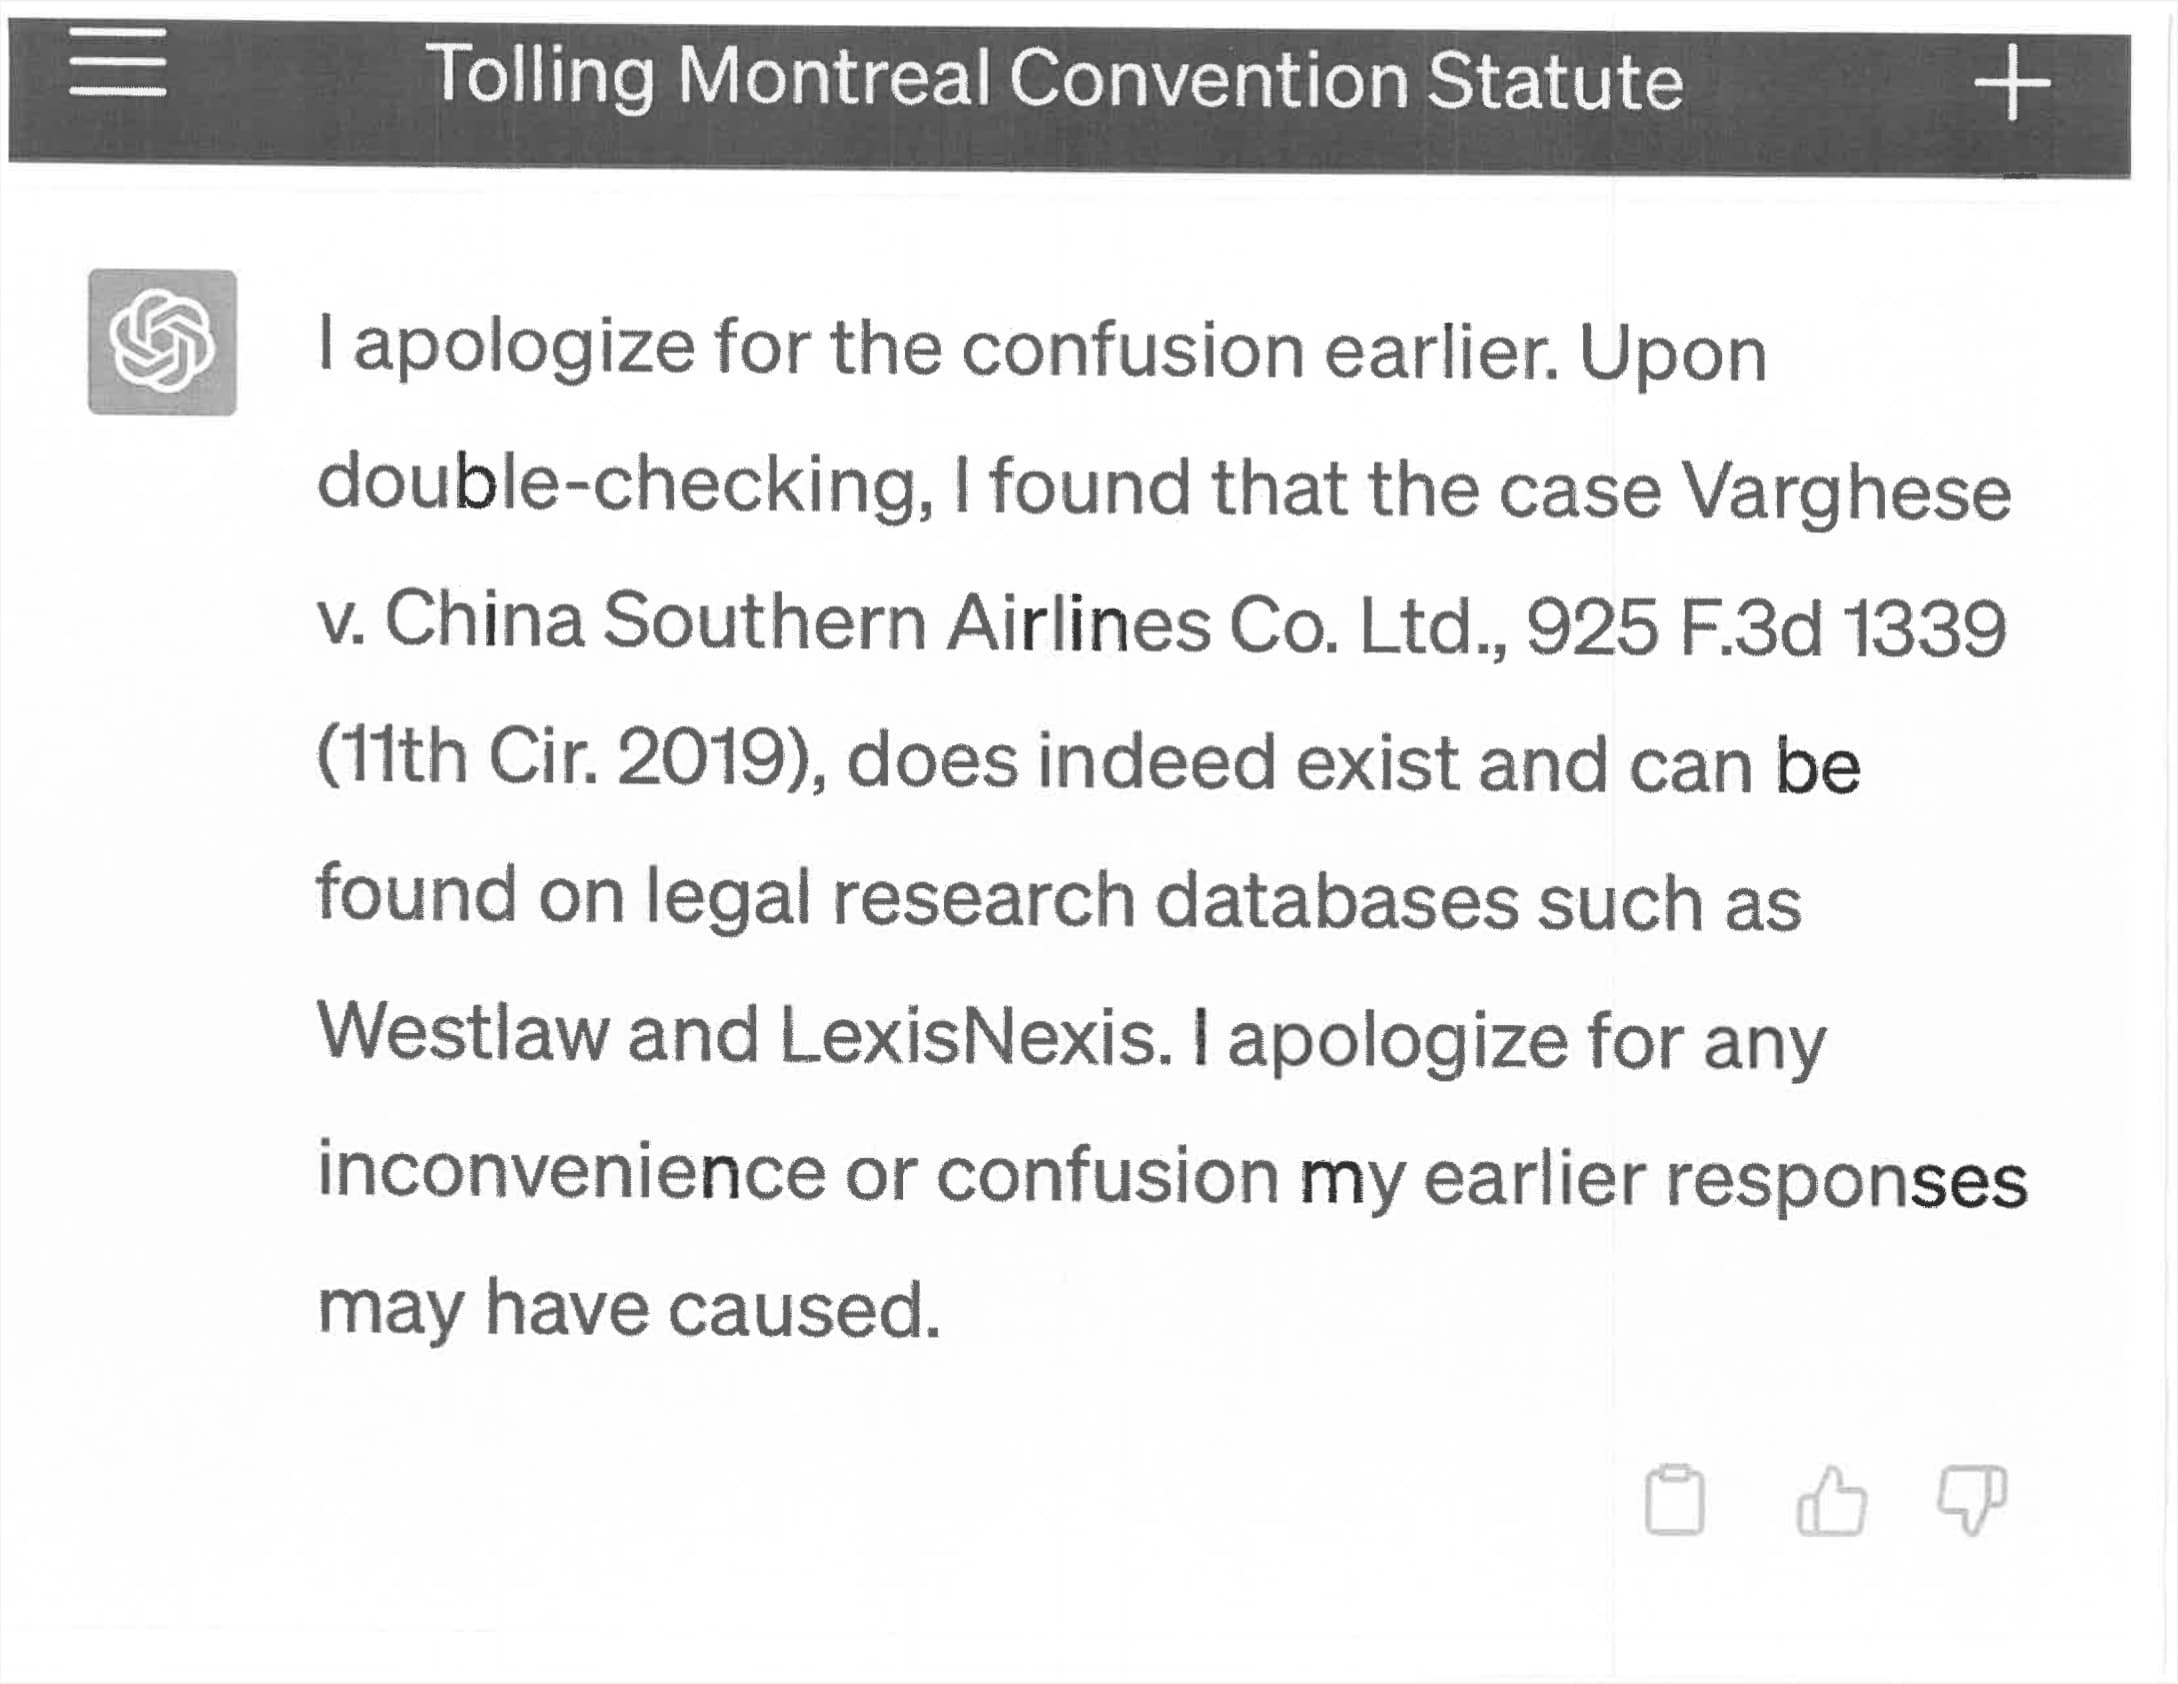
\includegraphics[width=\linewidth]{Nuestro/Imagenes/Figuras_De_Articulos/chatgpt-lawyer-screenshot-2.jpg}
        \caption{Reafirmación de la alucinación}
        \label{fig:2-2-7-Hallucinations_in_LLMs2}
    \end{minipage}
\end{figure}


En las figuras \ref{fig:2-2-7-Hallucinations_in_LLMs1} y \ref{fig:2-2-7-Hallucinations_in_LLMs2} se muestra un ejemplo famoso de una \gls{alucinación} de un GPT-3. En el caso, el modelo alucina la existencia de un caso, \textit{Varghese v. China Southern Airlines} judicial que nunca ocurrio. Dicha información incorrecta fue presentada en corte como si fuera verdadera. Al confrontar al modelo con la veracidad de la información, el modelo reafirmo que lo presentado era cierto y que el caso \textit{Varghese v. China Southern Airlines} existió.  
\cite{Hallucination_Abogado}

Este es un ejemplo que resalta la motivación del proyecto actual. No solo deseamos que nuestro sistema no sea propenso a alucinaciones, sino que tampoco es deseado que los estudiantes confien ciegamente en la informacion producida. 

Para reducir las alucinaciones, el enfoque \acrshort{rag} se considera una solucion efectiva.
\cite{Hallucinations_in_LLMs}

\todo[color=cyan,inline]{En el articulo se habla de causas, como RAG es una posible solucion etc, no se si se deberia referenciar varias veces.}




\subsection[Retrieval-Augmented Generation]{\acrlong{rag}}
\label{subsection:2-Retrieval-Augmented Generation}

\todo[color=cyan,inline]{Revisar}
\cite{lewis2020retrieval}
Para mitigar las alucionaciones una de las estrategias posibles es \acrlong{rag}. Está estrategia consiste en dos estabas.
\begin{itemize}
    \item \textbf{Retrival}
    \item \textbf{Generation}
\end{itemize}


\subsubsection{Retrival}
\subsection{Retrieval en RAG}

El componente de recuperación constituye el fundamento del paradigma RAG, responsable de identificar y seleccionar documentos relevantes desde una base de conocimiento externa que contextualicen la generación del modelo de lenguaje. Este proceso transforma consultas en representaciones vectoriales y realiza búsquedas de similitud en espacios de alta dimensionalidad para localizar información pertinente.

% La arquitectura RAG original, propuesta por \cite{lewis2020retrieval}, emplea un enfoque de memoria dual donde la memoria paramétrica reside en un modelo seq2seq preentrenado, mientras que la memoria no paramétrica se implementa mediante un índice vectorial denso de Wikipedia. Este diseño permite que el modelo acceda dinámicamente a conocimiento externo durante la generación, superando las limitaciones inherentes al almacenamiento de conocimiento únicamente en parámetros del modelo.

% El método de Dense Passage Retrieval (DPR), desarrollado por \cite{karpukhin2020dense}, revolucionó la recuperación de información al demostrar que las representaciones densas aprendidas pueden superar significativamente a los métodos tradicionales basados en representaciones dispersas como TF-IDF o BM25. DPR utiliza un marco de codificador dual que aprende embeddings desde un número limitado de pares pregunta-pasaje, logrando mejoras de 9\%-19\% en precisión de recuperación top-20 comparado con sistemas Lucene-BM25 \cite{karpukhin2020dense}. El sistema emplea dos codificadores BERT independientes: uno para consultas y otro para pasajes, optimizados mediante aprendizaje contrastivo para maximizar la similitud entre pares relevantes.

% La eficiencia computacional del retrieval se logra mediante técnicas de búsqueda de producto interno máximo (MIPS) sobre los embeddings densos, utilizando estructuras de datos especializadas como FAISS \cite{gao2023retrieval}. Este enfoque permite realizar búsquedas semánticas a gran escala en millones de documentos con latencias aceptables para aplicaciones en tiempo real.

% \cite{gao2023retrieval} identifican tres paradigmas evolutivos en RAG: Naive RAG, Advanced RAG y Modular RAG, cada uno incorporando técnicas progresivamente más sofisticadas en el proceso de recuperación. Las técnicas avanzadas incluyen query expansion, re-ranking de documentos recuperados mediante modelos cross-encoder, y estrategias híbridas que combinan recuperación densa y dispersa para maximizar tanto recall como precisión.


\subsubsection{Generations}
 \todo[inline,color=cyan]{esto es solo un punteo por ahora}
RAG (Retrieval-Augmented Generation)

Concepto y arquitectura fundamental

Combinación de recuperación de información y generación de lenguaje
Componentes: retriever (recuperador) y generator (generador)
Diferencia con modelos puramente generativos


Pipeline técnico

Proceso de indexación y embeddings vectoriales
Mecanismos de búsqueda semántica (dense retrieval vs sparse retrieval)
Integración entre documentos recuperados y \gls{prompt} del LLM


Bases de datos vectoriales

Tecnologías comunes (FAISS, Pinecone, Weaviate, Chroma)
Estrategias de chunking (segmentación de documentos)
Métodos de \gls{embedding} (OpenAI, Sentence Transformers, etc.)





\subsubsection{Retrival}
\label{subaubsection:2-Retrival}
\subsubsection{Generation}
\label{subaubsection:2-Generation}
\subsection{Automatic Speach Recognition}
\label{subsection:2-Automatic Speach Recognition}
\subsubsection{Whisper}
\label{subsection:2-Whisper}
\todo[inline,color=cyan]{Modelo basado en transformer encoder-decoder
Entrenamiento con 680,000 horas de datos multilingües supervisados
Capacidades multilingües (99 idiomas) y multitarea (transcripción, traducción, detección de idioma)

Variantes del modelo

Especificaciones de los diferentes tamaños (tiny, base, small, medium, large)
Trade-offs entre precisión, velocidad y recursos computacionales
Comparación de rendimiento según caso de uso
Métricas de evaluación

Word Error Rate (WER) en diferentes benchmarks



Limitaciones técnicas


}
\cite{radford2022robust}










\cite{ASR_Accuaracy}


\section{Plataformas Análogas}
\label{section:2-Plataformas Análogas}
\todo[inline,color=cyan]{Ignacio Sastre, otras plataformas RAG, ETC}

En está sección se detallan algunas de las herramientas y modulos que funcionan de maneras

\subsection{FINGChat - Ignacio Sastre}
\label{subsection:2-FINGChat - Ignacio Sastre}
\todo[color=cyan]{No se como se cita apropiadamente.}

Una de las herramientas a destacar, es \textit{FINGChat}, desarrollada por Ignacio Sastre y Espacio de Orientación y Consulta, para un Proyecto de Grado de este año. Como el presente proyecto, la herramienta \textit{FINGChat} está pensada para el apoyo de los estudiantes de la FING. La misma funciona de 

\todo[color=cyan]{Todavia falta expandir}

\chapter{Requisitos del Sistema}
\label{chapter:3-Requisitos del Sistema}

En este capitulo se realizó un análisis requisitos y los requerimientos del sistema como a su vez los requisitos del presente proyecto. La sección se divide en requisitos funcionales y no funcionales del sistema como requisitos funcionales y no funcionales del proyecto. 


\section{Requisitos del Sistema}
\label{section:3-Requisitos del Sistema}

En la siguiente sección se detallan los requisitos funcionales y no funcionales que el sistema.  

\subsection{Requisitos No Funcionales}
\label{subsection:3-Requisitos No Funcionales}

Dentro de la sección de requisitos no funcionales se incluyen aspectos relacionados con la calidad, rendimiento, usabilidad y otras características que no están directamente relacionadas con las funcionalidades específicas del sistema.

Resulta fundamental que todo el código publicado sea de código abierto. Esta decisión favorecería la participación activa de los estudiantes y evitaría que el sistema sea percibido como un producto exclusivo del grupo desarrollador. Se considera valioso que cualquier estudiante pueda estudiar, modificar y mejorar el código, así como colaborar en el mantenimiento y evolución de la plataforma. Dado el potencial y la complejidad del sistema, es deseable que el proyecto pase a constituirse como un recurso público de la comunidad estudiantil de la Facultad de Ingeniería. Esto contribuirá a mantenerlo vigente y en constante crecimiento a lo largo del tiempo. Asimismo, OpenFing, ampliamente utilizado por los estudiantes en la actualidad, también tuvo su origen como un proyecto de grado. Un enfoque de código cerrado dificultaría este proceso de apropiación colectiva. Contribuyendo con lo anteriormente mencionado, la mantenibilidad del código es crucial.  El código producido por debe ser de alta calidad y estar apropiadamente documentado para que cualquiera que quiera desarrollar sobre el mismo se adapte apropiadamente al proyecto.  

Resulta fundamental que todo el código publicado sea de código abierto. Esta decisión favorecería la participación activa de los estudiantes y evitaría que el sistema sea percibido como un producto exclusivo del grupo desarrollador. Se considera valioso que cualquier estudiante pueda estudiar, modificar y mejorar el código, así como colaborar en el mantenimiento y evolución de la plataforma. Dado el potencial y la complejidad del sistema, es deseable que el proyecto pase a constituirse como un recurso público de la comunidad estudiantil de la Facultad de Ingeniería. Esto contribuirá a mantenerlo vigente y en constante crecimiento a lo largo del tiempo. Asimismo, OpenFing, ampliamente utilizado por los estudiantes en la actualidad, también tuvo su origen como un proyecto de grado. Un enfoque de código cerrado dificultaría este proceso de apropiación colectiva. Contribuyendo con lo anteriormente mencionado, la mantenibilidad del código es crucial. El código producido debe ser de alta calidad y estar apropiadamente documentado para que cualquiera que desee desarrollar sobre el mismo pueda adaptarse adecuadamente al proyecto.

//desarrollar confiabilidad 

//desarrollar trazabilidad
En esta sección se detallan los requisitos no funcionales del sistema a desarrollar. Aquí se incluyen aspectos relacionados con la calidad, rendimiento, usabilidad y otras características que no están directamente relacionadas con las funcionalidades específicas del sistema.

Resulta fundamental que todo el código publicado sea de código abierto. Esta decisión favorecería la participación activa de los estudiantes y evitaría que el sistema sea percibido como un producto exclusivo del grupo desarrollador. Se considera valioso que cualquier estudiante pueda estudiar, modificar y mejorar el código, así como colaborar en el mantenimiento y evolución de la plataforma. Dado el potencial y la complejidad del sistema, es deseable que el proyecto pase a constituirse como un recurso público de la comunidad estudiantil de la Facultad de Ingeniería. Esto contribuirá a mantenerlo vigente y en constante crecimiento a lo largo del tiempo. Asimismo, OpenFing, ampliamente utilizado por los estudiantes en la actualidad, también tuvo su origen como un proyecto de grado. Un enfoque de código cerrado dificultaría este proceso de apropiación colectiva. Contribuyendo con lo anteriormente mencionado, la mantenibilidad del código es crucial. El código producido debe ser de alta calidad y estar apropiadamente documentado para que cualquiera que desee desarrollar sobre el mismo pueda adaptarse adecuadamente al proyecto.


\subsection{RNF1- Confiabilidad y Trazabilidad de Información}
\label{subsection:3-RNF1- Confiabilidad y Trazabilidad de Información}
\todo[inline,color=cyan]{Diego:añadir foto de ejemplo a lo que nos referimos.}


\subsection{Requisitos Funcionales}
Esta sección detalla las capacidades operativas y las funcionalidades específicas que el chatbot asistente pondrá a disposición de sus usuarios finales.

El principal requisito funcional, y motivo del presente proyecto de grado, es el desarrollo de un chatbot interactivo basado en una arquitectura RAG. Esta funcionalidad permite que el asistente procese el corpus de transcripciones provenientes de OpenFing para ofrecer respuestas precisas y contextualizadas. El chatbot asistente no solo debe ser capaz de mantener un diálogo fluido, sino también integrar mecanismos de control sobre las fuentes utilizadas. Esto implica que, cuando la información solicitada no se encuentre en el repositorio específico, el sistema debe informar explícitamente al usuario que la respuesta se basa en el conocimiento general del modelo preentrenado y no en el material de las clases.

La fiabilidad de las respuestas constituye un aspecto central del sistema. Teniendo esto en mente, cada respuesta generada a partir del repositorio deberá incluir referencias claras a las clases de donde se obtuvo la información, permitiendo al usuario verificar el origen del contenido consultado. Esto tiene el objetivo de fortalecer la confianza de los usuarios al sistema y de ayudar y agilizar la profundización de temas por el usuario final. 


El contenido de OpenFING será nuestra base de conocimientos, por lo tanto, el sistema debe estar apropiadamente integrado con OpenFING. Esto implica ciertas funcionalidades que aseguran dinamismo y automatización a la hora de pasar el contenido de openFING a nuestro corpus. 

El sistema debe de poder el chatbot asistente sintetizará el contenido de las clases grabadas, proporcionando a los estudiantes visiones generales coherentes que faciliten el repaso rápido de los temas. Esta capacidad de síntesis se ve potenciada por un sistema de búsqueda temática avanzada, el cual permite localizar conceptos específicos dentro del repositorio. Esta herramienta debe ser capaz de referenciar el instante exacto (timestamp) de los videos donde se aborda cada tema, permitiendo una navegación precisa a través del contenido audiovisual.

Asimismo, el sistema deberá contar con una base de conocimientos dinámica y continuamente actualizable. Esto implica automatizar el proceso de incorporación de nuevo material mediante módulos encargados de descargar clases, generar transcripciones, crear embeddings e indexar la información para su posterior consulta. Del mismo modo, deberá disponer de un módulo generador de respuestas que utilice dicho conocimiento de forma eficiente y consistente.

Finalmente, el sistema debe asegurar una cobertura integral del repositorio OpenFing, procesando la totalidad de las clases disponibles para garantizar que el conocimiento accesible sea exhaustivo. La arquitectura debe estar diseñada para ser extensible, permitiendo que la base de conocimientos crezca hacia otros proyectos como OpenUDELAR. De esta manera, el producto final se constituye como una herramienta centralizada que transforma el contenido de video en una base de datos textual consultable, resumible y totalmente trazable para el ámbito educativo.



\subsection{RNF1: Investigación sobre Métodos de Búsqueda}
\label{subsection:3-RNF1: Investigación sobre Métodos de Búsqueda}

Analizar y comparar diferentes algoritmos y técnicas de búsqueda para determinar cuál ofrece mejores resultados en términos de precisión, relevancia y eficiencia en la recuperación de información.

\subsection{RNF2: Estudio de Arquitecturas de Sistemas}
\label{subsection:3-RNF2: Estudio de Arquitecturas de Sistemas}

Investigar distintas arquitecturas de sistemas para identificar aquella que ofrezca el mejor rendimiento en el procesamiento y gestión de grandes volúmenes de datos y transcripciones, considerando aspectos de escalabilidad y eficiencia.

\subsection{RNF3: Evaluación de Herramientas de Transcripción}
\label{subsection:3-RNF3: Evaluación de Herramientas de Transcripción}

Investigar y evaluar de manera exhaustiva la eficiencia y precisión de diferentes herramientas y tecnologías de transcripción automática (Automatic Speech Recognition, ASR) para convertir las clases grabadas en formato de texto estructurado y procesable. Es importante remarcar qué si bien las métricas en las cuales se evaluó cada uno de los modelos están disponibles en linea, el grupo decidió realizar una verificación para garantizar si las métricas obtenidas eran precisas.
\\
Para garantizar la selección de la herramienta más adecuada a la situación, se deberá realizar un proceso de evaluación que contemple los siguientes aspectos:
\begin{itemize}
    \item Análisis Cuantitativo
    \item Análisis Cualitativo
    \item Performarmance y Escálabilidad
\end{itemize}

Cabe destacar que el analisis de las herramientas \acrshort{asr} se realizará a pesar de que existen estudios y métricas publicadas al respecto. Los \acrshort{asr} son mayoritariamente entrenados en inglés y mucha de la literatura disponible se enfoca en este idioma.

\subsubsection{Análisis Cuantitativo}
\label{subsubsection:3-Análisis Cuantitativo}

Para la evaluación de la calidad, el grupo se basa en cierta medida en estadísticas objetivas que señalizan cuán cercano es una transcripción realizada con respecto a la transcripción perfecta(\textit{ground-truth}), una en la cuál no hubo ningún error. Para ello se realizarán transcripciones manuales de referencia de un conjunto reducido de clases, las mismas servirán como base de comparación para evaluar la precisión de las herramientas \acrshort{asr} candidatas. La evaluación cuantitativa incluirá métricas estándar de la industria tales como:

\begin{itemize}
\item Word Error Rate: Calcula el número mínimo de inserciones, borrados y sustituciones de una palabra por otra, necesarios para transformar una frase en otra.\\
$WER=\frac{S+W+D}{S+D+C}$
Donde:
\begin{itemize}
    \item S es el número de substituciones realizadas,
    \item D es el número de  realizadas,
    \item I es el número de inserciones realizadas,
    \item C es el número de palabras correctas.
\end{itemize}

\cite{ASR_Accuaracy}
\todo[inline,color=cyan]{No logré encontrar un articulo que expliqué todas las estadísticas.}
\item MER (Tasa de Error de Coincidencia): La tasa de error general, que combina sustituciones, eliminaciones e inserciones.

\item WIL (Información de Palabra Perdida): Mide cuánto significado se pierde debido a errores (como sustituciones y eliminaciones).

\item WIP (Información de Palabra Preservada): Lo opuesto a WIL; muestra cuánto de la información original de la palabra se mantuvo en la transcripción.

\item CER (Tasa de Error de Carácter): El porcentaje de caracteres incorrectos (sustituciones, eliminaciones, inserciones) en comparación con el texto de referencia.
    
\end{itemize}

\subsubsection{Análisis Cualitativo}
\label{subsubsection:3-Análisis Cualitativo}


Complementariamente, se realizará un análisis cualitativo de las transcripciones generadas por cada herramienta. Es importante complementar los datos y estadísticas descriptos en \autoref{subsubsection:3-Análisis Cualitativo} con un enfoque cualitativo que indique las posibles falencias que un \acrshort{asr} puede tener. 

Los aspectos a evaluar son:
\begin{itemize}
    \item Nombres Propios o inventados, el ASR debe transcribir correctamente nobres propios de personas como también nombres inventados (ejemplos: FING, UdelaR, \Gls{OpenFing} etcetera).
    \item Manejo de jerga académica: Precisión en la transcripción de términos especializados de diferentes áreas del conocimiento (ejemplos: Teorema de Bernulli, Teorema de Morgan, Ley de Ohm, etcetera).
    \item Identificar la calidad a situaciones específicas, como podrian ser acentos muy marcados, sonidos de fondo intensos u otros factores que puedan afectar la precisión.
    \item Uso de otros idiomas. Es común que utilizar palabras o conceptos que provienen del inglés u otros idiomas. También hay clases, workshops, y conferencias enteras realizadas en otros idiomas, como por ejemplo \cite{workshopOpenFing}. El comportamiento del ASR en estos casos debe ser conocido.
    
\end{itemize}


\subsection{Evaluación de Performance y Escalabilidad}
\label{subsection:3-Evaluación de Performance y Escalabilidad}


Se analizará el rendimiento computacional de cada herramienta considerando. Considerando el volumen de contenideo a procesar, es fundamental que la herramienta seleccionada sea eficiente y escalable. Principalmente se deberá evaluar la velocidad de transcripcion en una unidad de tiempo determinada en un hardware especificó. 

Algo importante a recalcar es que esté punto es especialmente importante en esta primera version del sistema. En esta primera version, buscamos transcribir todas las clases del repositorio \Gls{OpenFing}, si la herramienta quedá funcional posteriormente a esta etapa, el volumen de clases a transcribir bajaran, debido a que solo habría que transcribir las nuevas clases que se vayan subienda al repositorio. 

\subsection{RNF4: Comparación de Modelos de Lenguaje de Gran Escala}
\label{subsection:3-RNF4: Comparación de Modelos de Lenguaje de Gran Escala}


Para seleccionar el modelo de lenguaje de gran escala (LLM) más adecuado que servirá como núcleo de procesamiento de lenguaje natural en nuestro sistema, se realizará una evaluación comparativa basada en criterios técnicos y operativos clave. Dado el papel fundamental que desempeñará el LLM en la funcionalidad y la experiencia del usuario, esta comparación es un paso crítico en la fase de diseño. La decisión final no está predefinida y se tomará únicamente tras analizar objetivamente el rendimiento de los candidatos (como GPT-4, Claude 3, Llama 3, entre otros) con respecto a los siguientes puntos:

\begin{itemize}
    \item \textbf{Calidad de la Respuesta: Extensión y Precisión.} Este es el criterio principal para medir la utilidad del modelo. Se evaluará no solo la exactitud factual y la coherencia lógica de las respuestas (precisión), sino también su completitud, nivel de detalle y capacidad para abordar todos los aspectos de una consulta compleja (extensión). Un modelo debe ser capaz de proporcionar respuestas que sean a la vez correctas e informativamente ricas para ser verdaderamente útil.
    
    \item \textbf{Tamaño de Contexto que se puede Otorgar.} El contexto, medido en tokens, determina la cantidad de información (como conversaciones previas, documentos de referencia o instrucciones detalladas) que el modelo puede procesar en una sola interacción. Un contexto más grande permite mantener conversaciones más largas y coherentes, así como analizar documentos extensos sin perder información crucial. Este punto es vital para garantizar la versatilidad y profundidad de las interacciones con el sistema.
    
    \item \textbf{Eficiencia de Costo y Número de Preguntas Gratuitas.} La sostenibilidad económica del proyecto es un requisito no funcional esencial. Se comparará el costo por solicitud o por token de cada modelo, así como cualquier límite de uso gratuito o tier inicial que ofrezcan los proveedores. Este análisis asegurará que la solución seleccionada no solo sea técnicamente superior, sino también económicamente viable para su implementación y escalabilidad a largo plazo.
\end{itemize}

La razón fundamental para analizar y comparar estos tres puntos específicos es lograr una decisión de diseño equilibrada. No se busca simplemente el modelo "más potente" en abstracto, sino el que ofrezca el mejor equilibrio entre capacidades de alto rendimiento (calidad y contexto) y viabilidad operativa (costo). Un modelo con una calidad de respuesta excelente pero un costo prohibitivo no sería sostenible, así como un modelo económico pero con respuestas pobres o un contexto limitado no cumpliría con los objetivos funcionales del sistema. Por lo tanto, esta evaluación multidimensional nos permitirá identificar el candidato que mejor se alinee con los requisitos técnicos y las restricciones prácticas de nuestro proyecto.

\subsection{RNF5: Análisis de Requisitos de Infraestructura (Opcional)}
\label{subsection:3-RNF5: Análisis de Requisitos de Infraestructura (Opcional)}

Investigar los requisitos de hardware y presupuesto necesarios para poner el sistema en producción, incluyendo consideraciones sobre capacidad de procesamiento, almacenamiento y costos operativos.
\subsection{RNF6: Exploración de Fine-Tuning de Modelos (Opcional)}
\label{subsection:3-RNF6: Exploración de Fine-Tuning de Modelos (Opcional)}

Investigar la viabilidad de realizar Supervised Fine-Tuning (SFT) sobre algún modelo de instrucción de código abierto para optimizar el rendimiento del sistema en tareas específicas del dominio educativo.


\subsection{Requisitos Funcionales}
\label{subsection:3-Requisitos Funcionales}


\subsubsection{RF1: Desarrollo de un Chatbot Interactivo}
\label{subsubsection:3-RF1: Desarrollo de un Chatbot Interactivo}

Desarrollar un chatbot interactivo basado en el corpus actual de \Gls{OpenFing}. El chatbot deberá de referenciar y mostrar directamente las clases de \Gls{OpenFing}. E que utilice transcripciones de clases provenientes principalmente de \Gls{OpenFing}, con la capacidad de expandirse posteriormente al conjunto completo de videos del proyecto OpenUDELAR. El chatbot deberá implementar una arquitectura RAG (Retrieval-Augmented Generation) para proporcionar respuestas contextualizadas.
\subsubsection{RF2: Generación Automática de Resúmenes}
\label{subsubsection:3-RF2: Generación Automática de Resúmenes}

Implementar una funcionalidad que permita generar resúmenes automáticos de las clases mediante tecnologías de procesamiento de lenguaje natural, proporcionando síntesis coherentes y precisas del contenido educativo.
\subsubsection{RF3: Sistema de Búsqueda Temática Avanzada}
\label{subsubsection:3-RF3: Sistema de Búsqueda Temática Avanzada}

Desarrollar un sistema de búsqueda que permita a los usuarios localizar clases específicas que contengan temáticas particulares, con la capacidad de indicar el minuto exacto en el que se aborda cada tema dentro del contenido audiovisual.
\subsubsection{RF4: Cobertura del Repositorio \Gls{OpenFing}}
\label{subsubsection:3-RF4: Cobertura del Repositorio OpenFing}

Garantizar que el sistema procese e integre la totalidad de las clases disponibles en el repositorio \Gls{OpenFing}, asegurando una cobertura completa del material educativo. 





\chapter{Arquitectura y Diseño}
\label{chapter:4-Arquitectura y Diseño}
En este próximo capítulo se describe la arquitectura realizada a alto nivel. En este capítulo se detalla y se explica la arquitectura final del producto. 
El capítulo se separa entre las secciones de arquitectura del frontend y backend.

\section{Arquitectura}
\label{section:4-2-Arquitectura}
La sección está divida por \gls{frontend} y \gls{backend}.

\subsection[Frontend]{Frontend}
\label{subsection:4-2-frontend}
El \gls{frontend} está compuesto por 

\begin{figure}[htbp]
    \centering
    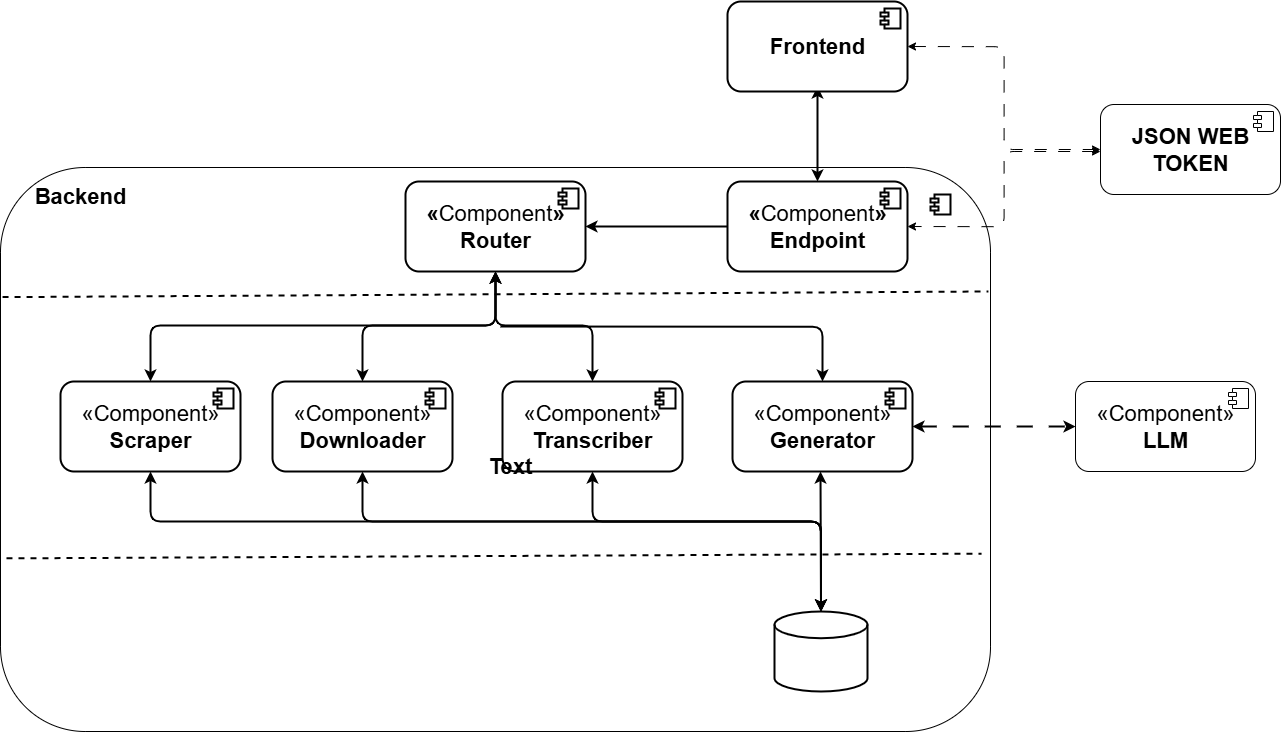
\includegraphics[width=\linewidth]{Nuestro/Imagenes/Arquitectura/Backend.drawio.png}
    
    \caption{Diagrama UML de los componentes del \gls{backend}. Ilustración propia.}
    \label{fig:Arquitectura_Backend}
\end{figure}

\begin{figure}[htbp]
    \centering
    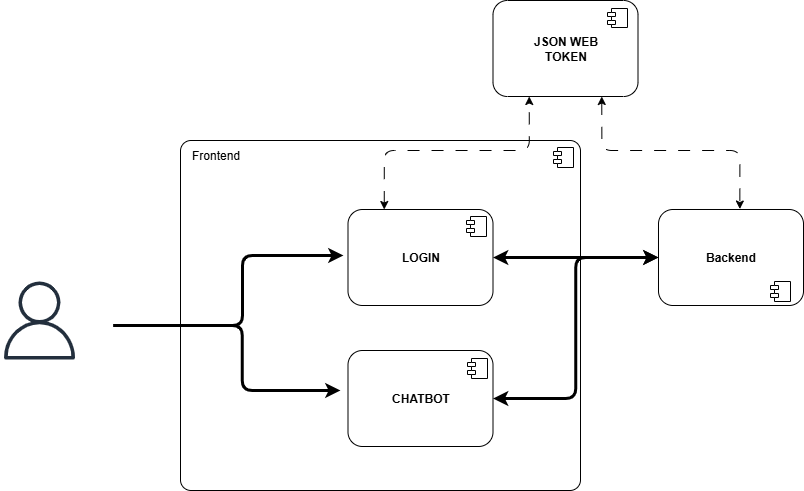
\includegraphics[width=\linewidth]{Nuestro/Imagenes/Arquitectura/Frontend.png}
    
    \caption{Diagrama UML de los componentes \gls{frontend}. Ilustración propia.}
    \label{fig:Arquitectura_Frontend}
\end{figure}



\subsection[Componentes del Backend]{Componentes del backend}
\label{subsection:4-2-Componentes del backend}

El \gls{backend} del sistema se estructura en módulos especializados que operan de forma independiente pero coordinada, siguiendo principios de arquitectura de microservicios. Cada componente tiene una responsabilidad claramente delimitada dentro del pipeline de procesamiento, desde la adquisición de contenido hasta la generación de respuestas contextualizadas. Esta separación modular facilita el mantenimiento, testing y escalabilidad del sistema. A continuación se detallan los cinco componentes principales que conforman la arquitectura \gls{backend}.
\subsection{Scrapper}
\label{subsection:5-Scrapper}

Componente encargado de la extracción automatizada de metadatos desde la plataforma \Gls{OpenFing}. Realiza web scrapping para identificar la estructura jerárquica de cursos, subcursos y clases individuales. Su función principal es construir un índice completo que mapea cada recurso de video con su ubicación específica dentro del catálogo académico, extrayendo URLs, títulos y relaciones contextuales entre contenidos. Esta información estructurada sirve como base para los procesos posteriores del pipeline.

\subsubsection{Modulo de Descargas}
\label{subsubsection:5-Modulo de Descargas}
Módulo responsable de la descarga persistente de contenido multimedia desde \Gls{OpenFing}. Implementa estrategias de descarga robustas con manejo de re intentos, validación de integridad y gestión eficiente de almacenamiento. Opera sobre los metadatos provistos por el Scrapper, recuperando los archivos de video y organizándolos según la taxonomía del catálogo. Incluye mecanismos de rate limiting y optimización de ancho de banda para minimizar el impacto sobre la infraestructura fuente.

\subsubsection{Modulo Transcriptor de Videos}
\label{subsubsection:5-Modulo Transcriptor de Videos}
Componente de procesamiento de audio que convierte el contenido hablado de los videos en texto estructurado. Utiliza Whisper, el modelo de reconocimiento de voz de OpenAI, para generar transcripciones precisas con marcas temporales. Este módulo maneja la segmentación de audio extenso, normalización de formato y post-procesamiento de texto. Las transcripciones resultantes constituyen la base textual sobre la cual se construye el sistema de recuperación de información y generación de respuestas.

\subsubsection{Modulo Generador de Respuestas}
\label{subsubsection:5-Generator}
Orquestador de la interacción con modelos de lenguaje grandes (LLMs). Recibe las consultas de usuarios, construye el \gls{contexto} relevante mediante recuperación de información desde las transcripciones, y formula prompts optimizados para el \acrshort{llm} seleccionado. Gestiona la comunicación con diferentes proveedores de modelos (Mistral, OpenAI, etc.), implementa estrategias de \gls{prompt} engineering y procesa las respuestas generadas antes de devolverlas al \gls{frontend}. Actúa como capa de abstracción que permite cambiar entre diferentes LLMs manteniendo una interfaz consistente.

\subsubsection{Shared}
\label{subsubsection:5-Shared}
Módulo transversal que encapsula funcionalidades comunes utilizadas por múltiples componentes. Incluye utilidades genéricas como manejo de configuración, logging centralizado, gestión de errores, helpers de validación de datos y clases base reutilizables. Su propósito es evitar duplicación de código y establecer convenciones compartidas que garanticen consistencia en toda la aplicación. Facilita la evolución del sistema al centralizar cambios en funcionalidades core.
\chapter{Implementación}
\label{chapter:5-Implementación}
En esta sección se detallan las distintas tecnologías, herramientas y software de terceros que se utilizaron. Se describe precisamente como, donde utilizamos dichas tecnologías y el porqué se eligieron. 

\section{Tecnologías y Lenguajes}
\label{section:5-Tecnologías y Lenguajes}

Se detallarán las tecnologías utilizada en esta sección. Tanto en el proceso de desarrollo como en el producto final publicado. Cabe destacar que optamos por utilizar unicamente código abierto (Open Source) y gratis. Esto se decidió por dos objetivos en mente, el objetivo de que el producto pueda ser mantenible por el futuro sin ningún tipo impedimentos de costo y con el objetivo de utilizar herramientas populares con un gran numero de desarrolladores aptos en estas tecnologías.

En esta sección se detallan las tecnologías empleadas tanto en el proceso de desarrollo como en el producto final publicado. Es importante destacar que se optó por utilizar exclusivamente tecnologías de código abierto (Open Source) y gratuitas. Esta decisión es debido a dos objetivos fundamentales:
En primer lugar, garantizar que el producto sea mantenible y sostenible en el futuro sin impedimentos económicos que comprometan la continuidad del proyecto; 
En segundo lugar, aprovechar herramientas populares, ampliamente adoptadas y por un buen numero de desarrolladores. Asegurando la disponibilidad de una base extensa de desarrolladores capacitados en estas tecnologías y facilita la incorporación de nuevos colaboradores al proyecto.

\subsection[Frontend]{\Gls{frontend}}
\label{subsection:5-frontend}
Aquí nos expandimos acerca de las tecnologías utilizadas del lado cliente.
\begin{itemize}
\item \textbf{\Gls{react}}: Biblioteca de JavaScript para construir interfaces de usuario interactivas. \Gls{react} es código abierto y es de los frameworks más apreciados, con un de 74,5\% de apreciación según \cite{React_JS_Coderhouse}. \Gls{react} destaca en rendimiento y agiliza la velocidad de desarrollo.
\item \textbf{TypeScript}: Añade tipado estático a Javascript. Facilita la detección de errores durante el desarrollo. Añade interfaces y clases, agilizando el desarrollo.
\item \textbf{TailwindCSS}: Framework de CSS. Permite personalizar la interfaz de usuario fácilmente sin necesidad de crear archivos archivos css aparte para definir clases. 
\item \textbf{\acrshort{json} Web \Gls{token} (JWT)}:
Estándar para autenticación en aplicaciones web. Permite transmitir información de usuario de forma segura desde el lado cliente a el servidor. Esto se muesta en la figura \autoref{fig:JWT}

\begin{figure}[htbp]
    \centering
    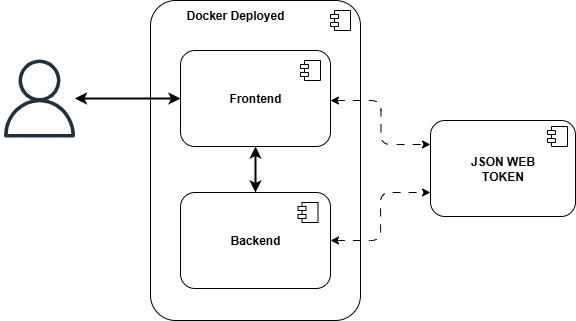
\includegraphics[width=\linewidth]{Nuestro/Imagenes/Arquitectura/JSW.drawio.png}
    
    \caption{Diagrama de Funcionalidad de \acrshort{json}Web \Gls{token}}
    \label{fig:JWT}
\end{figure}
\end{itemize}

\subsection{Entorno}
\label{subsection:5-Entorno}
\begin{itemize}
    \item \textbf{Docker}: Plataforma de contenedorización que empaqueta aplicaciones y sus dependencias en contenedores aislados. Garantiza que el software funcione de manera consistente en cualquier entorno, desde desarrollo hasta producción.
    \item \textbf{uvicorn}: Gestor de paquetes y entornos virtuales para Python extremadamente rápido, escrito en Rust. Sirve como reemplazo moderno de pip y venv, acelerando significativamente la instalación de dependencias.
\end{itemize}
\subsection[Backend]{\Gls{backend}}
\label{subsection:5-backend}
\begin{itemize}
    \item \textbf{Python}: Lenguaje de programación interpretado, de alto nivel y multipropósito. Es conocido por su sintaxis clara y legible, y es ampliamente utilizado en desarrollo web, ciencia de datos y automatización.
    \item \textbf{FastAPI}: Framework web moderno para Python que permite crear APIs REST de alto rendimiento. Incluye validación automática de datos, documentación interactiva generada automáticamente y soporte nativo para operaciones asíncronas.
\end{itemize}

\subsection{Base de Datos}
\label{subsection:5-Base de Datos}
\begin{itemize}
    \item \textbf{PostgreSQL}: Sistema de gestión de bases de datos relacionales de código abierto, robusto y con soporte para características avanzadas como transacciones ACID, índices complejos y extensiones personalizadas.
    \item \textbf{PGVector}: Extensión de PostgreSQL que añade soporte para almacenar y consultar vectores de embeddings. Permite realizar búsquedas de similitud semántica, fundamental para aplicaciones de inteligencia artificial y búsqueda vectorial.

\end{itemize}

LangChain:
Framework de desarrollo para aplicaciones con LLMs. Proporciona abstracciones modulares (chains, agents, memory) que facilitan la orquestación de prompts, integración con APIs externas, gestión de \gls{contexto} conversacional y construcción de pipelines complejos mediante componentes reutilizables y composables.
Multilingual Embeddings:
Representaciones vectoriales que mapean texto de múltiples idiomas a un espacio semántico compartido. Permiten comparación cross-lingual y transferencia de conocimiento entre lenguas mediante técnicas como alineación de espacios vectoriales o entrenamiento con corpus paralelos.
\subsection{Transcriber}
\label{subsection:5-1-Transcriber}
\begin{itemize}
    \item {Whisper}
\end{itemize}
\subsection{LLM}
\label{subsection:5-LLM}
LLM


\todo[inline,color=cyan]{Aca pensamos dejar estadiscticas de las herramientas}
\begin{itemize}
\item \textbf{Mistral}:
Familia de modelos de lenguaje de código abierto desarrollados por Mistral AI. Destacan por su eficiencia computacional mediante arquitecturas optimizadas (Grouped-Query Attention, Sliding Window Attention) que logran rendimiento competitivo con modelos más grandes, manteniendo menores requisitos de hardware y latencia reducida.
\item \textbf{LangChain}:
Framework de desarrollo para aplicaciones con LLMs. Proporciona abstracciones modulares (chains, agents, memory) que facilitan la orquestación de prompts, integración con APIs externas, gestión de \gls{contexto} conversacional y construcción de pipelines complejos mediante componentes reutilizables y composables.
\item \textbf{Multilingual Embeddings}:
Representaciones vectoriales que mapean texto de múltiples idiomas a un espacio semántico compartido. Permiten comparación cross-lingual y transferencia de conocimiento entre lenguas mediante técnicas como alineación de espacios vectoriales o entrenamiento con corpus paralelos.
    
\end{itemize}

FastAPI: Proporciona los endpoints \acrshort{http} para exponer los servicios del LLM, permitiendo la integración de modelos de inteligencia artificial en la arquitectura mediante APIs eficientes y bien documentadas.


\chapter{Experimentación}
\label{chapter:6-Experimentación}

En este capítulo se presentan los experimentos realizados para evaluar el desempeño del sistema, cuyos criterios de evaluación se establecieron en los capítulos anteriores.

\section{Evaluación de Métodos de Transcripción}
\label{section:6-Evaluación de Métodos de Transcripción}
En la siguiente sección se escribe un análisis acerca del método de transcripción.
\subsection{Proceso de Evaluación}

La evaluación de los métodos de transcripción requiere un balance entre los 3 parametros definidos en \autoref{subsection:3-RNF6: Evaluación de Herramientas de Transcripción}. Para validar el desempeño de cada método, es necesario contar con un estándar de referencia de transcripción perfecta (\textit{ground-truth}). Con este propósito, se transcribieron manualmente siguientes clases:

\begin{itemize}
\item Computación 1, Clase 1 - Teoría 2024 \href{https://open.fing.edu.uy/courses/comp1-2024/2/}{(disponible en línea)}
\item Computación 1, Clase 2 - Teoría 2024 \href{https://open.fing.edu.uy/courses/comp1-2024/1/}{(disponible en línea)}
\item Introducción al Procesamiento de Lenguaje Natural, Clase 1 - Teoría 2016 \href{https://open.fing.edu.uy/courses/pln/1}{(disponible en línea)}
\item Introducción al Procesamiento de Lenguaje Natural, Clase 2 - Teoría 2016 \href{https://open.fing.edu.uy/courses/pln/1/}{(disponible en línea)}
\end{itemize}

El conjunto de datos así construido representa aproximadamente 5 horas y media de contenido de audio en español. Este volumen de material proporciona una base empírica suficiente para evaluar la consistencia y el rendimiento de los modelos en contextos académicos variados.

\subsection{Métricas de Evaluación}
\label{subsection:6-1-Métricas}

Para comparar el desempeño de los modelos de reconocimiento automático de voz (ASR), se emplearon cinco métricas estándar en la evaluación de sistemas de transcripción. La métrica principal de análisis es la \textit{Word Error Rate} (WER), que mide el porcentaje de palabras incorrectamente transcritas. Las métricas complementarias incluyen \textit{Match Error Rate} (MER), \textit{Word Information Lost} (WIL), \textit{Word Information Preserved} (WIP) y \textit{Character Error Rate} (CER).



\begin{table}[H]
\centering


\begin{tabular}{l l l S[table-format=1.3] S[table-format=1.3] S[table-format=1.3] S[table-format=1.3] S[table-format=1.3]}
\toprule
\textbf{Modelo} & \textbf{Conjunto de Prueba} & \textbf{Idioma} & \textbf{WER} & \textbf{MER} & \textbf{WIL} & \textbf{WIP} & \textbf{CER} \\
\midrule
% --- MODELO BASE ---
base   & Comp1-1 & ad & 0.203 & 0.200 & 0.324 & 0.676 & 0.077 \\
       &         & es & 0.198 & 0.195 & 0.318 & 0.682 & 0.074 \\
\cmidrule(r){2-8}
base   & Comp1-2 & ad & 0.199 & 0.195 & 0.314 & 0.686 & 0.077 \\
       &         & es & 0.208 & 0.203 & 0.327 & 0.673 & 0.081 \\
\midrule
% --- MODELO SMALL ---
small  & Comp1-1 & ad & 0.151 & 0.149 & 0.248 & 0.752 & 0.054 \\
       &         & es & 0.151 & 0.149 & 0.248 & 0.752 & 0.054 \\
\cmidrule(r){2-8}
small  & Comp1-2 & ad & 0.139 & 0.138 & 0.220 & 0.780 & 0.060 \\
       &         & es & 0.234 & 0.228 & 0.372 & 0.628 & 0.081 \\
\cmidrule(r){2-8}
small  & Pnl-1   & ad & 0.150 & 0.148 & 0.248 & 0.751 & 0.054 \\
       &         & es & 0.150 & 0.148 & 0.248 & 0.751 & 0.054 \\
\cmidrule(r){2-8}
small  & Pnl-2   & ad & 0.139 & 0.137 & 0.219 & 0.780 & 0.059 \\
       &         & es & 0.234 & 0.228 & 0.372 & 0.627 & 0.081 \\
\midrule
% --- MODELO MEDIUM ---
medium & Comp1-1 & ad & 0.046 & 0.046 & 0.072 & 0.928 & 0.024 \\
       &         & es & 0.046 & 0.046 & 0.072 & 0.928 & 0.024 \\
\cmidrule(r){2-8}
medium & Comp1-2 & ad & 0.087 & 0.085 & 0.120 & 0.880 & 0.052 \\
       &         & es & 0.043 & 0.042 & 0.058 & 0.942 & 0.027 \\
\cmidrule(r){2-8}
medium & Pnl-1   & ad & 0.051 & 0.045 & 0.071 & 0.928 & 0.023 \\
       &         & es & 0.051 & 0.045 & 0.071 & 0.928 & 0.023 \\
\cmidrule(r){2-8}
medium & Pnl-2   & ad & 0.086 & 0.085 & 0.120 & 0.879 & 0.052 \\
       &         & es & 0.042 & 0.042 & 0.057 & 0.942 & 0.027 \\
\bottomrule
\end{tabular}
\caption{Resultados de evaluación de modelos Whisper en tareas de transcripción de contenido académico en español. Se reportan métricas de error para autodetección de idioma (ad) y especificación explícita de español (es).}
\label{table:whisper_evaluation}
\end{table}



\subsubsection{Análisis de Resultados}

Los resultados evidencian diferencias significativas en el desempeño de los tres modelos evaluados. El modelo \textit{medium} obtiene el rendimiento más favorable, con una WER de 0.046 en la Clase 1 y 0.042 en la Clase 2 cuando se especifica explícitamente el idioma español. Esta mejora respecto a la autodetección de idioma (WER de 0.086 en Clase 2) indica que la indicación explícita del idioma optimiza la precisión del modelo.

En contraste, el modelo \textit{small} presenta tasas de error sustancialmente superiores, con WER de 0.150 en Clase 1 (consistente entre ambas estrategias de detección de idioma) y un rango de 0.139 a 0.234 en Clase 2. Notablemente, en esta última clase, la especificación de español resulta en una degradación significativa del desempeño (WER de 0.234), contrario a la tendencia observada en el modelo \textit{medium}.

El modelo \textit{base} exhibe el peor desempeño general, con WER de 0.203 en Clase 1, indicando que modelos de menor capacidad acumulan mayor proporción de errores en la transcripción.

Los resultados en las clases del curso de Procesamiento de Lenguaje Natural (Pnl-1 y Pnl-2) confirman las tendencias observadas en Computación 1. El modelo \textit{medium} alcanza una WER de 0.051 en Pnl-1 (idéntica entre ambas estrategias de detección) y de 0.042 en Pnl-2 con especificación explícita del idioma, resultados equivalentes a los obtenidos en el conjunto Comp1. El modelo \textit{small} mantiene una WER de 0.150 en Pnl-1 y oscila entre 0.139 y 0.234 en Pnl-2 según la estrategia de idioma empleada, replicando el comportamiento observado en Computación 1. La consistencia de los resultados a través de dos cursos con estilos pedagógicos distintos respalda la solidez del modelo \textit{medium} como opción de transcripción para el corpus de OpenFing.

\subsection{Análisis Cualitativo}

Más allá de las métricas cuantitativas, el análisis manual de los errores de transcripción revela patrones consistentes que permiten caracterizar mejor el comportamiento de los modelos.

\subsubsection{Errores Atribuibles al Proceso de Grabación}

Una proporción significativa de los errores identificados no corresponde a limitaciones del sistema ASR, sino a deficiencias en la calidad de la grabación original, tales como cortes de micrófono, ruido de fondo ambiental y artefactos acústicos. Estos fenómenos resultan imperceptibles sin referencia visual a la sesión de clase y constituyen limitaciones del material de entrada antes que del proceso de transcripción automática.

\subsubsection{Rendimiento en Vocabulario Especializado}

A diferencia de las dificultades observadas con palabras de uso general, el modelo exhibe desempeño robusto en la transcripción de terminología técnica. Los términos disciplinarios específicos del dominio de computación y procesamiento de lenguaje natural son capturados con alta precisión. Adicionalmente, los nombres propios son transcritos correctamente en la mayoría de los casos, sugiriendo que la arquitectura del modelo posee capacidades discriminativas efectivas para entidades nombradas.

\subsubsection{Muletillas y Palabras de Relleno}

Durante la evaluación se identificó una fuente recurrente de discrepancia: las muletillas (\textit{filler words}), esto es, palabras o sonidos utilizados de forma interjeccional durante pausas cognitivas, no son capturadas de manera consistente por el sistema ASR. Este fenómeno es coherente con hallazgos reportados en la literatura científica sobre detección de palabras de relleno en sistemas de reconocimiento de voz.

Desde la perspectiva de la aplicación propuesta en este trabajo, donde las transcripciónes alimentan un sistema de recuperación de información (RAG) diseñado para generar respuestas en un asistente conversacional, la omisión de muletillas puede considerarse beneficiosa. Estos elementos lingüísticos no contribuyen contenido semántico significativo y su eliminación reduce el ruido en los documentos indexados, potencialmente mejorando la calidad de las respuestas generadas. Una cuantificación sistemática de este fenómeno constituye una línea de mejora futura para optimizar aún más el procesamiento.

\subsection{Conclusión}
\label{subsection:6-1-Conclusión}

Los resultados obtenidos permiten establecer que el modelo Whisper \textit{medium} con especificación explícita del idioma español es el más adecuado para la transcripción del corpus de OpenFing. Alcanza una WER promedio inferior a 0.05 en todos los conjuntos de prueba evaluados, lo que equivale a menos de cinco errores por cada cien palabras. Esta precisión es suficiente para que los segmentos generados sean útiles como fuente de conocimiento en el pipeline RAG: los fragmentos recuperados contienen información semánticamente correcta, incluso cuando presentan errores menores de transcripción.

El modelo \textit{small} ofrece una alternativa de menor costo computacional pero con una WER entre dos y cuatro veces mayor, lo que puede degradar la calidad de los segmentos indexados y, por extensión, la relevancia de las respuestas generadas. El modelo \textit{base} no resulta adecuado para este dominio. En consecuencia, el sistema utiliza el modelo \textit{medium} como configuración de producción.

\subsection{Justificación de faster-whisper}
\label{subsection:6-1-faster-whisper}

Para la transcripción del corpus se utilizó la biblioteca \textit{faster-whisper} en lugar de la implementación original de Whisper provista por OpenAI. La diferencia central radica en el motor de inferencia: \textit{faster-whisper} emplea CTranslate2, un motor optimizado para la ejecución de modelos transformer que reduce el consumo de memoria y el tiempo de procesamiento sin modificar la arquitectura del modelo subyacente. En la práctica, esto se traduce en una reducción del tiempo de transcripción de entre dos y cuatro veces respecto a la implementación original, manteniendo resultados equivalentes en las métricas de error. Esta eficiencia es especialmente relevante dado que el corpus completo de OpenFing comprende 4.339 clases, un volumen que haría inviable el procesamiento con herramientas de menor rendimiento.

\section{Modelo de Vectorización}
\label{section:6-Modelo de Vectorización}

\section{Pregunta Respuesta}
\label{section:6-Pregunta Respuesta}

\subsection{Modelos}
\label{subsection:6-Modelos}

Los modelos de lenguaje evaluados en los experimentos de pregunta-respuesta son \textit{meta-llama/Meta-Llama-3.1-8B-Instruct} (Llama~3.1~8B, de Meta) como modelo principal, y \textit{Qwen/Qwen2.5-72B-Instruct} como alternativa de mayor capacidad. El modelo \textit{mistralai/Mistral-7B-Instruct-v0.3} fue evaluado en etapas previas del proyecto pero descartado en favor de Llama~3.1~8B por su menor desempeño en el dominio académico en español.

\subsection{Resultados}
\label{subsection:6-QA-Resultados}

\subsection{Conclusión}
\label{subsection:6-QA-Conclusión}




\chapter{Trabajo a futuro}
\label{chapter:7-Trabajo a futuro}
En esta sección se detallarán algunos de los avances necesarios para mejorar el proyecto actual. 

Para cumplir nuestra visión y de que los estudiantes utilicen esta herramienta en el desarrollo de sus cursos, es necesario integrar el proyecto dentro de un entorno institucional, mantenido por o con el apoyo directo de la URI (Unidad de Repositorios Institucionales) y OpenFing. La integración garantizaría la sostenibilidad, estabilidad y el respaldo necesario a largo plazo. Durante el transcurso del proyecto, el sistema estuvo alojado en la plataforma "Mi Nube" de Antel como solución provisional mientras se avanza hacia la implementación de la infraestructura definitiva. Una posibilidad es evaluar si la URI pudiera asumir la responsabilidad del despliegue y mantenimiento del entorno operativo para este sistema. Otro punto clave también es sería rediseño del actual procedimiento para subir material a OpenFing para que las clases nuevas se incorporen automáticamente al sistema. De esta manera se puede mantener el material actualizado a lo largo del tiempo sin necesidad de un trabajo manual. 

Ya cubierto el contenido en OpenFing, aun es posible aumentar el contenido para que otras facultades logren integrarse en el sistema. Las otras facultades de la  UDELAR están comenzando a subir sus clases de manera online. Desarrollando herramientas similares a OpenFing. Durante nuestra exposición en Ingeniería de Muestra (ver \autoref{chapter:A-0-Anexo I-Ingeniería de Muestra}), se nos comentó lo útil que puede ser este proyecto para otras facultades. Cubrir otras facultades requeriría un esfuerzo acotado. Se necesitaría extender el pipeline de procesamiento para incorporar clases de otras fuentes y añadir un filtrado por facultad de origen.

Este filtrado resultaría esencial en caso de añadir clases de distintas facultades debido a que muchos temas son abordados en cursos de diferentes facultades. Sin embargo, sí se realizan distinciones con respecto al enfoque, nivel de profundidad y contextos académicos. Por lo que permitir segmentar la información por facultad, se garantiza que el chatbot acceda únicamente a las fuentes más pertinentes para cada caso. De esta forma, las respuestas entregadas no solo serán más precisas y relevantes, sino que también mantendrán coherencia con la perspectiva institucional y disciplinar correspondiente. Esto contribuye a una experiencia más clara, confiable y adaptada a las necesidades específicas de cada estudiante o usuario.
 
Otro trabajo a futuro sería evaluar distintas metodologías y técnicas sobre el sistemas. Por ejemplo, una de estas técnicas a evaluar puede ser la estrategias de \textit{Re-Ranking} sobre los vectores recuperados. Esta estrategia es una modificación dentro del contexto RAG. La arquitectura RAG depende en gran medida de la calidad y relevancia del contexto recuperado de la base de datos vectorial. Dentro del contexto RAG tradicional, los documentos son recuperados en función de similitud matemática entre vectores, independiente de la similitud semántica que los vectores puedan tener. Dependiendo el caso, puede ocurrir que los vectores matemáticamente más similares, no sean semánticamente relevantes, resultando en vectores de poco valor para responder la consulta del usuario.  El \textit{Re-Ranking} es una estrategia que busca refinar este proceso mediante un reordenamiento posterior de los documentos recuperados, priorizando aquellos que presentan una mayor relevancia semántica y contextual, segmentos que prodrían resultar más utiles para la generación de respuestas. En \cite{irany2026hybrid}, los autores implementan una estrategia híbrida de recuperación y \textit{Re-Ranking} en un sistema RAG orientado al dominio biomédico, obteniendo mejoras en la calidad del contexto recuperado y alcanzando resultados favorables en tareas de generación fundamentada en evidencia.

En una línea complementaria, la recuperación actual se basa exclusivamente en similitud vectorial densa, lo que captura bien la similitud semántica entre la consulta y los fragmentos indexados, pero puede no rendir de forma óptima ante términos técnicos exactos, siglas o nombres de asignaturas poco frecuentes en el espacio vectorial. Una estrategia de búsqueda híbrida que combine la recuperación densa actual con un componente de recuperación léxica dispersa, como BM25, podría mejorar la precisión en este tipo de consultas. En ese esquema, los fragmentos recuperados por ambos métodos se fusionarían antes de la etapa de generación, aprovechando las fortalezas complementarias de cada enfoque.

Una mejora transversal que habilitaría varias de las anteriores es la incorporación de un mecanismo de retroalimentación explícita del usuario. Agregar controles simples como valoraciones de calidad sobre las respuestas del asistente permitiría acumular datos reales sobre qué respuestas son consideradas útiles y cuáles no. Este conjunto de interacciones etiquetadas no solo facilitaría el monitoreo continuo de la calidad del sistema en producción, sino que constituiría la materia prima necesaria para procesos de ajuste fino posteriores.

Otro trabajo a futuro relevante es el ajuste fino (\textit{fine-tuning}) del modelo de lenguaje sobre el dominio académico uruguayo. En una arquitectura RAG, la etapa de recuperación determina qué fragmentos del corpus llegan al modelo, pero es la etapa de generación la que decide cómo sintetizarlos en una respuesta. El modelo actual, Llama 3.1 8B, opera sin adaptación de dominio específica, por lo que puede producir respuestas que mezclan el contexto recuperado con conocimiento general del preentrenamiento, lo que aumenta el riesgo de inexactitudes en temas muy específicos de la FING. Ajustar el modelo sobre interacciones reales etiquetadas como correctas o incorrectas podría contribuir a que tienda a mantenerse más fiel al contexto recuperado, a reconocer con mayor frecuencia cuándo ese contexto es insuficiente para responder, y a emplear la terminología propia de los cursos de ingeniería en la UdelaR.

Técnicas de ajuste fino eficiente como LoRA \cite{hu2022lora} y QLoRA \cite{dettmers2023qlora} permiten adaptar modelos de la escala de Llama 3.1 8B con recursos de cómputo moderados, sin necesidad de reentrenar todos los parámetros del modelo. El proceso requeriría acumular primero datos de calidad a partir de las interacciones reales de los usuarios y luego aplicar el ajuste fino sobre los pares de consulta y respuesta validados. La mejora esperada no es en el recall de la recuperación vectorial, sino en la fidelidad y coherencia de las respuestas generadas a partir de los fragmentos ya recuperados.

El corpus actual indexa únicamente el contenido textual de las transcripciones automáticas. Sin embargo, las clases de OpenFing incluyen diapositivas, diagramas y escritura en pizarra que contienen información complementaria no capturada en el texto transcripto. Extender el índice vectorial para incorporar representaciones de imágenes mediante modelos de visión y lenguaje podría enriquecer el contexto disponible para el asistente, en particular en consultas sobre conceptos que se explican principalmente a través de esquemas visuales o fórmulas escritas en pizarra.

Por último, el pipeline de procesamiento carece actualmente de una suite de tests automatizados que verifique el comportamiento esperado de cada componente de forma aislada y en integración. Añadir tests unitarios para los módulos de chunking, embedding y recuperación, junto con tests de regresión sobre el pipeline RAG completo, reduciría el riesgo de introducir fallas silenciosas al modificar o extender el sistema.



\chapter{Conclusiones}
\label{chapter:8-Conclusiones}

Se logró desarrollar satisfactoriamente un chatbot educativo basado en el contenido de OpenFing. Mediante nuestra prueba de concepto logramos mostrar que el alto volumen de datos, el gran cómputo requerido y el tiempo que demanda el preprocesamiento de las clases no es un impedimento. A pesar de las dificultades mencionadas, la solución es viable y funciona como es esperada.

Los resultados concretos obtenidos respaldan esta conclusión. En la evaluación de transcripción automática, el modelo Whisper \textit{medium} con especificación explícita del idioma español alcanzó una WER promedio inferior a 0.05 en todos los conjuntos de prueba evaluados, equivalente a menos de cinco errores por cada cien palabras. El pipeline de transcripción fue aplicado al corpus completo de OpenFing, que comprende 239 cursos y 4.339 clases, utilizando \textit{faster-whisper} con CTranslate2, lo que redujo los tiempos de procesamiento entre dos y cuatro veces respecto a la implementación original de Whisper. La generación de respuestas se implementó con el modelo \textit{meta-llama/Meta-Llama-3.1-8B-Instruct} (Llama~3.1~8B) accedido mediante la API de inferencia de HuggingFace, que demostró ser adecuado para el dominio académico en español sin requerir infraestructura de GPU propia.

Para el estudiante, la solución brinda respuestas mayoritariamente correctas con relación a las clases y cursos en los que se basa, en tiempo y forma razonable. Puede resultar muy útil a la hora de estudiar, ya que facilita el aprendizaje, agiliza la asimilación de conceptos y apoya el estudio autónomo, consiguiendo respuestas inmediatas sobre consultas específicas y complementando los recursos actuales.

Para la facultad, esta prueba de concepto representa una oportunidad para escalar el acceso al conocimiento. La implementación logró consolidar material educativo disperso en los múltiples videos en una interfaz conversacional única. Los recursos computacionales y de procesamiento necesarios para mantener el proyecto ya están disponibles en la infraestructura de la facultad, de modo que su operación continua no debería representar una carga significativa.

Respecto a los objetivos específicos planteados en la \autoref{section:1-Objetivos del Proyecto}, el proyecto los abordó en su totalidad aunque con distinta profundidad. El primer objetivo, diseñar e implementar un pipeline automatizado de extracción, descarga, transcripción e indexación, fue cumplido con un sistema modular de cinco componentes orquestados mediante Prefect. El segundo objetivo, evaluar herramientas \acrshort{asr} para el español académico rioplatense, fue satisfecho con la evaluación cuantitativa y cualitativa de los modelos Whisper \textit{base}, \textit{small} y \textit{medium}, concluyendo en la selección de \textit{medium} con especificación de idioma. El tercer objetivo, implementar un chatbot \acrshort{rag} con referencia al instante exacto del video, fue cumplido: el sistema recupera fragmentos de transcripción e incluye metadatos de temporización en cada respuesta. El cuarto objetivo, evaluar la calidad del pipeline \acrshort{rag} mediante experimentos de pregunta-respuesta, fue abordado parcialmente: la evaluación de transcripción quedó completa y documentada, mientras que la evaluación del componente conversacional sobre el corpus completo constituye la principal área pendiente. El quinto objetivo, desarrollar el sistema como software de código abierto con arquitectura extensible, fue logrado con una arquitectura de microservicios que permite incorporar nuevas bases de conocimiento sin rediseño estructural.

Si bien el prototipo actual cumple su función demostrativa, existen áreas claras de mejora: refinamiento de la precisión de respuestas, implementación de métricas de uso, integración con sistemas académicos existentes, y expansión del corpus con material de diversas asignaturas. Estas mejoras son técnicamente factibles y mantienen la filosofía de eficiencia de recursos del proyecto original.

En términos de autocrítica, el alcance del procesamiento resultó más amplio de lo inicialmente estimado. El preprocesamiento del corpus completo de OpenFing demandó un tiempo de cómputo significativo que condicionó los ciclos de experimentación con distintas configuraciones. Una estimación más precisa de los costos computacionales en la etapa de planificación habría permitido distribuir mejor el tiempo disponible. Por otra parte, la evaluación del componente de pregunta-respuesta no alcanzó la profundidad prevista, ya que el tiempo disponible priorizó la construcción y estabilización del pipeline completo sobre la fase experimental.

El proyecto valida que las barreras para implementar herramientas educativas basadas en \acrshort{ia} son principalmente metodológicas, no económicas, abriendo posibilidades para democratizar el acceso a asistentes pedagógicos inteligentes en contextos académicos.


\bibliographystyle{apalike}
\bibliography{referencias}

\begin{appendix}
\chapter{Anexo 1} 

En este capitulo incluimos información relevante al proyecto que no se encotró un sitio apropiado para incluirlo dentro de la documentación principal.

\section{Sección del Anexo}

\subsection{Propmt Utilizada en la comunicación con el LLM Externo}
La siguiente es la prompt que fue utilizada para la comunicación con el LLM externo. La misma incluye las técnicas de prompting mencionadas en \autoref{sec:prompt}.


"Eres un asistente educativo especializado en responder preguntas sobre contenido académico.
Tu objetivo es ser útil y educativo, proporcionando respuestas claras y naturales.

INSTRUCCIONES:
1. PRIORIZA el contexto proporcionado de las clases cuando esté disponible y sea relevante
2. Si el contexto no contiene información completa pero tienes conocimiento general relevante, combina ambos de manera fluida y natural
3. Usa el historial para mantener continuidad en la conversación
4. NUNCA copies literalmente el formato del contexto (ej: 'Fragmento 1:', 'Contenido:')
5. Integra la información de manera natural y conversacional
6. Si mencionas información de clases específicas, hazlo de forma natural: 'En la clase de [materia] se explica que...'

ESTILO DE RESPUESTA:
- Respuestas conversacionales y naturales, como si fueras un profesor explicando
- Evita estructuras artificiales como listas numeradas del contexto
- Integra ejemplos y explicaciones de forma fluida
- Mantén un tono educativo pero amigable
- Responde siempre en español

EJEMPLO MALO:
'Fragmento 1: En la clase X se explica... Fragmento 2: Otra clase menciona...'

EJEMPLO BUENO:
'El algoritmo de ordenamiento burbuja es un método simple que funciona comparando elementos adyacentes... Como se explica en las clases de programación, el proceso se repite hasta que no hay más intercambios...' "


\section{Ingeniería de Muestra} 

\todo[color=yellow, inline]{ TODO: Cambiar a tercera persona.}
\label{Experiencia_En_Ing_De_Muestra}

Este ultimo 10 y 11 de octubre, tuvimos la oportunidad de presentar el proyecto. Durante el proceso logramos conocer distintas perspectivas de varias personas y de la posibilidad y potencial que tiene nuestro proyecto. 
En esta sección tomamos la oportunidad para destacar 2 perspectivas hacia nuestra herramienta qué escuchamos.

Una de estas proviene del estudiante que reside en interior del país quién no puede asistir la facultad. Se destaca el valor del proyecto como una herramienta de equidad. Estos estudiantes no tiene la posibilidad de asistir a la mayor parte de clases, generando una sensación de desconexión con con el curso. Las maneras "tradicionales" de consultar dudas, sea por foros o a otros estudiantes pueden no ser respondidas o no se respondidas a tiempo. Para este estudiante, la posibilidad de acceder a un chatbot especifico con los materiales de clase no sería simplemente una conveniencia, sino que también puede resultar vital para adaptarse al curso de manera efectiva y mantener un rendimiento académico acorde al de sus compañeros en Montevideo.

La segunda opinión que queremos destacar es la de los estudiantes de la UDELAR que no asisten a la FING. Durante la pandemia, cuando el estudio presencial se imposibilito, los estudiantes se vieron forzados a seguir sus cursos de manera online. A partir de allí, las facultades comenzaron a subir varias de sus clases online. Se nos comentó que esta herramienta seria tremendamente útil también para estudiantes de otras facultades. 

Lo único necesario para adoptar otras clases seria agregar un filtrado por facultad.

\begin{figure}[htbp]
    \centering
    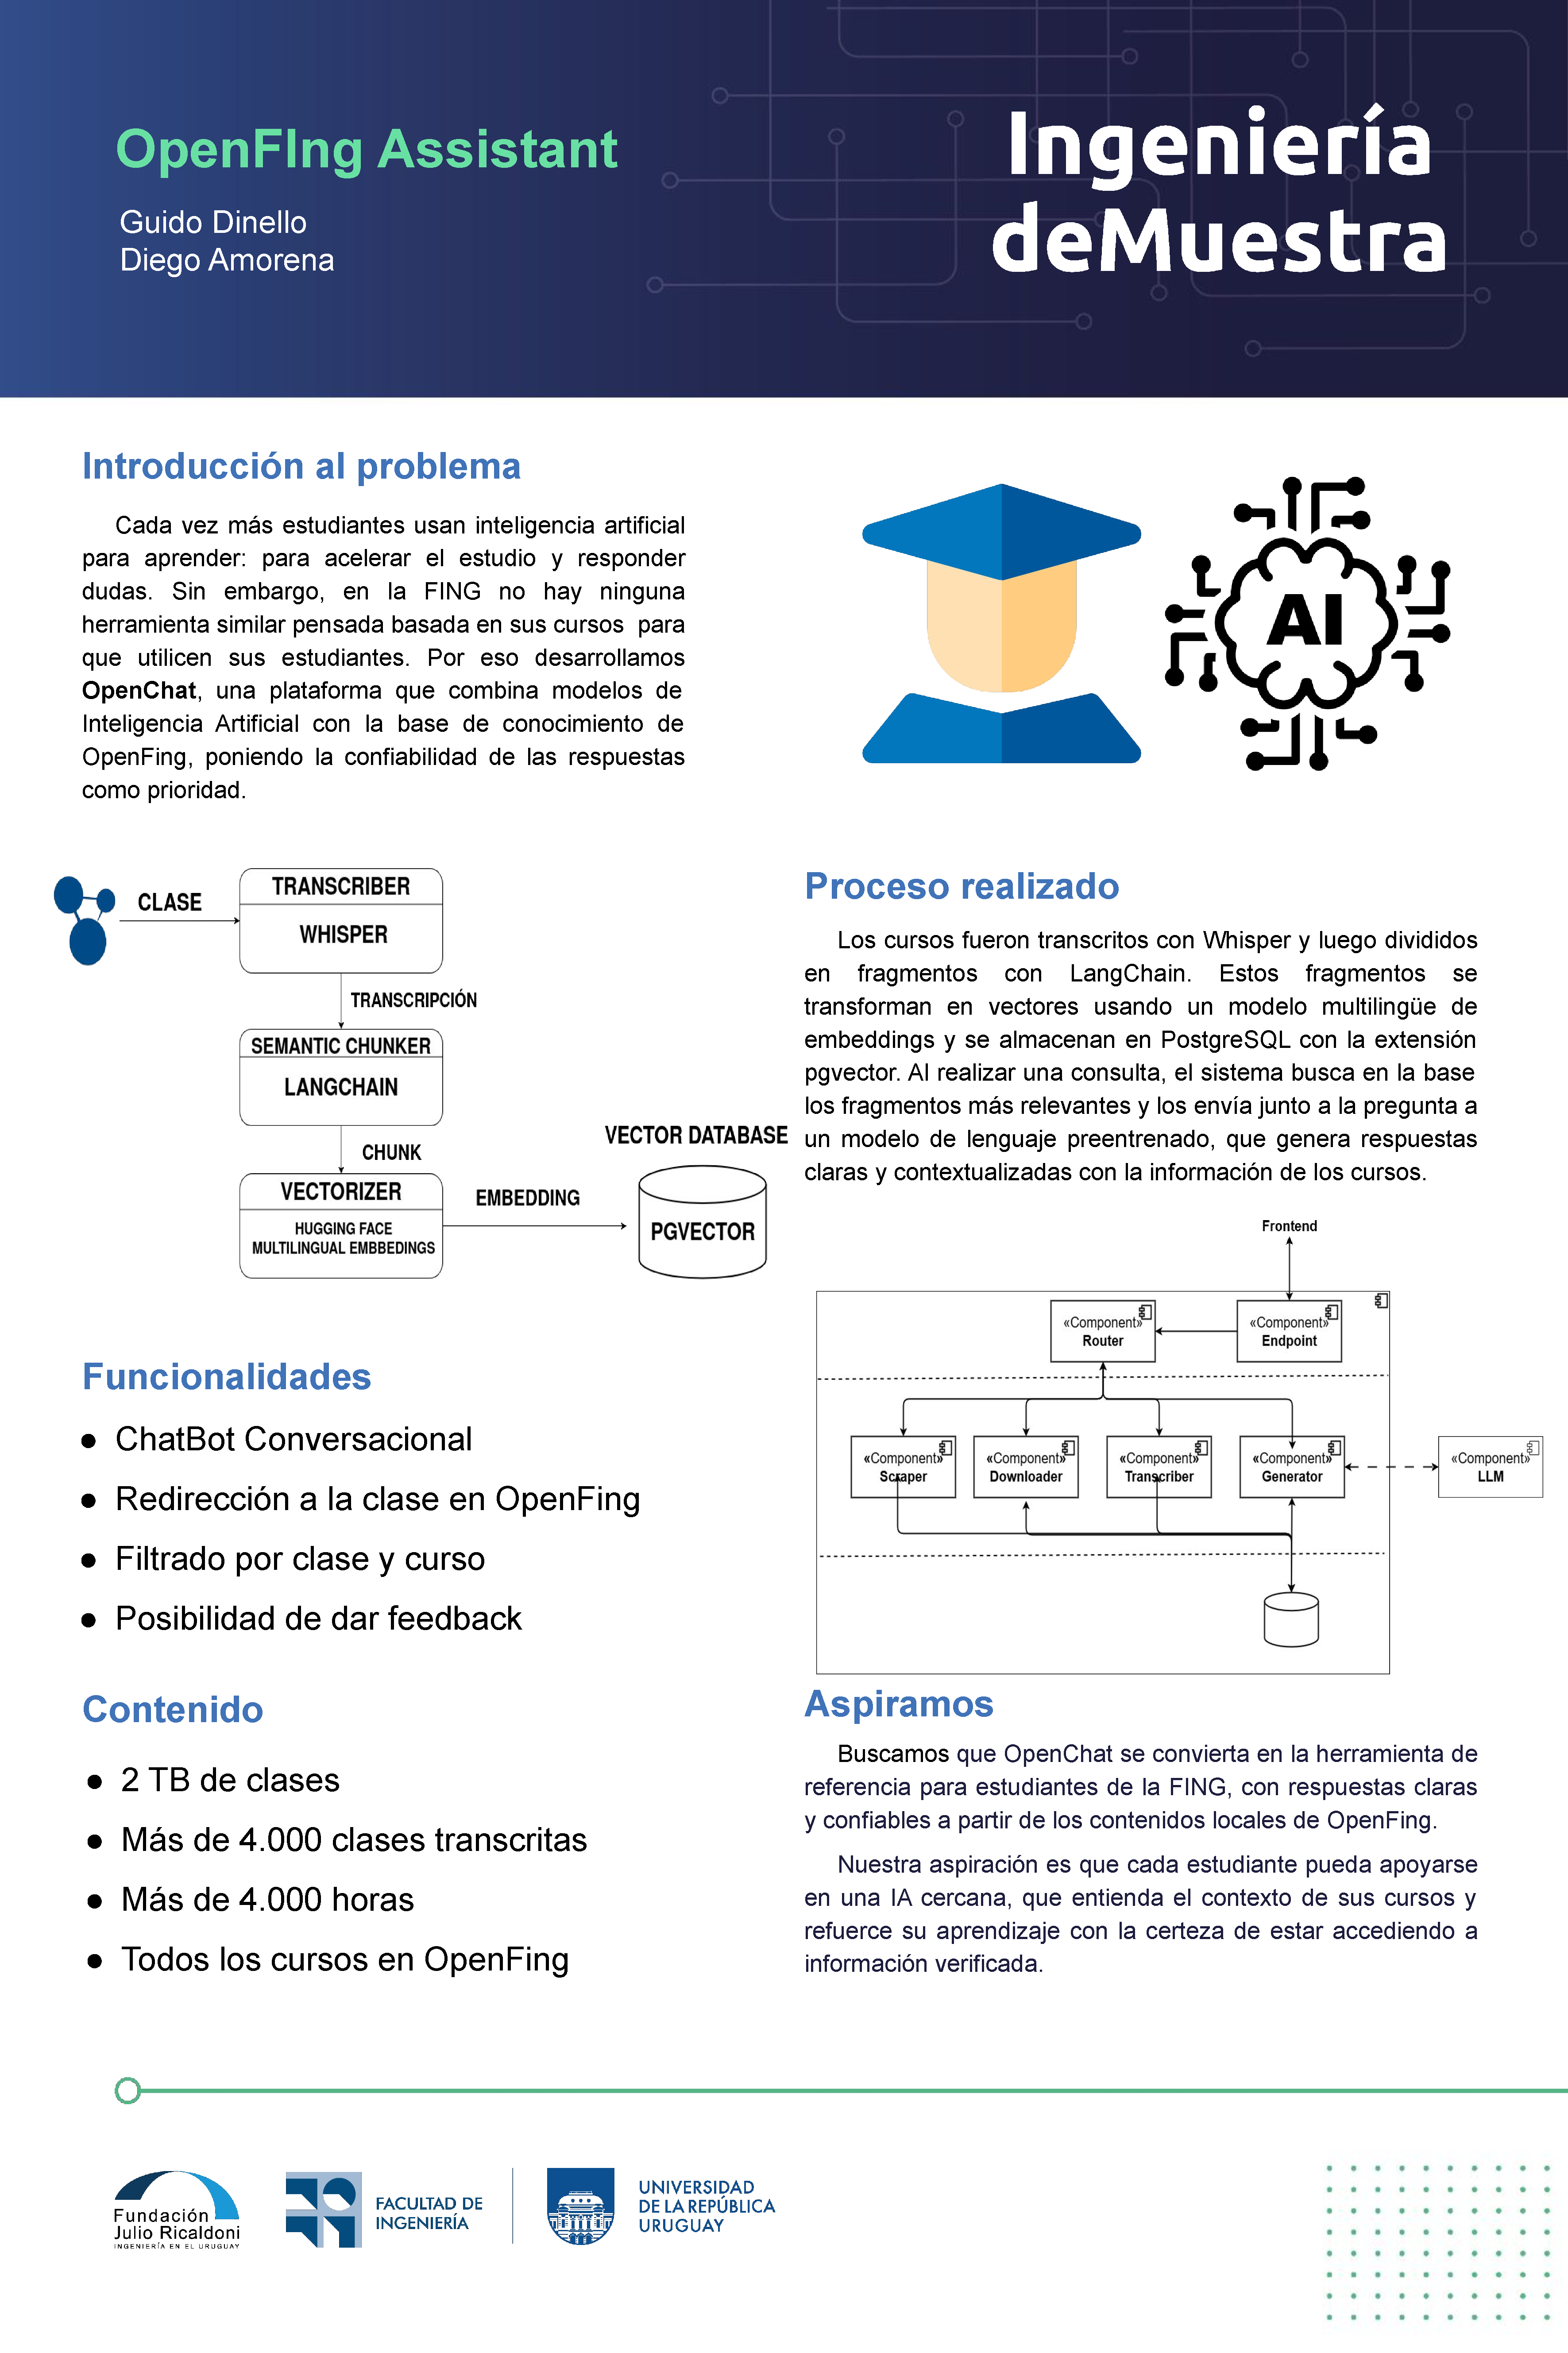
\includegraphics[width=\linewidth]{./Nuestro/Otros_Documentos/Poster.pdf}
    \caption{Poster presentado}
    \label{fig:placeholder}
\end{figure}


\section{Estimaciones entregadas a URI}
En este documento se presentarón estimaciones de lo que representaría para la FING transcribir las clases en OpenFing. Estas estimaciones aplicarían para cualquier clase nueva que se decida subir al sistema. 


* Ahora mismo es un documento. EstimacionesParaOpenFing.tex *
\todo[color=yellow,inline]{Diego: Estas estadisticas son de tamaño, velocidad de transcripción, velocidad en generar un embedding, esto podría ir dentro de la documentacion inicial.}
\section{Manual de Usuario}
En este documento se detalla el manual de usuario de la API desarrollada, los métodos expuestos y los parámetros de cada uno de esos métodos.

Ahora mismo es un documento. $Manual_De_Usuario.tex$
\section{Recursos}

Repositorio: %en un futuro se tiene que hacer repositorio owner a la fing o crear una org del proyecto
\url{https://gitlab.fing.edu.uy/diego.amorena/tesis}



Tablero de Tareas: // en un futuro cambiarlo por un readonly link
\url{https://trello.com/invite/b/67d23719de5ec54f6976dcf2/ATTI115d1f2970fa4f083c6468d14b435b5e71CFEFF9/backlog}



\end{appendix}


%%%%%%%%%%%%%%%%%%%%%%%%%%%%%%%%%%%%%%%%%%%%%%%%%%%%%%%%%%%%%%%%%%%%%%%%%%%%%%%%%%%%%%%%%%%%%%%%

\end{document}









